\documentclass[12pt, openany]{report}
\usepackage[utf8]{inputenc}
\usepackage[T1]{fontenc}
\usepackage[a4paper,left=2cm,right=2cm,top=1cm,bottom=2cm]{geometry}
\usepackage[french]{babel}
\usepackage{libertine}
\usepackage[pdftex]{graphicx}
\usepackage[export]{adjustbox}
\usepackage{setspace}
\usepackage{hyperref}
\usepackage{enumitem}
\usepackage[nottoc]{tocbibind}
\usepackage{amsmath,diagbox,tabu}
\usepackage{caption}
\usepackage{float}
\usepackage[Sonny]{fncychap}
\setcounter{tocdepth}{3}
\setcounter{secnumdepth}{3}


\hypersetup{
    colorlinks=true,
    linkcolor=black,
    filecolor=magenta,      
    urlcolor=blue,
}
\setstretch{1,4}
\setlength{\parindent}{4ex}
\setlength{\parskip}{1ex plus 0.5ex minus 0.2ex}
\newcommand{\hsp}{\hspace{20pt}}
\newcommand{\HRule}{\rule{\linewidth}{0.5mm}}

\newlist{mylist}{itemize}{3}
\setlist[mylist,1]{
    label=\textbullet,
    wide=0pt,
    itemindent=\dimexpr\parindent+\labelwidth+\labelsep\relax}

\begin{document}
\begin{titlepage}
  \begin{sffamily}
  \begin{center}

	\begin{figure}[t]
	   \begin{minipage}{0.48\textwidth } 
	     
\includegraphics[width=.3\linewidth , left]{ensias.JPG}
	   \end{minipage}\hfill
	   \begin{minipage}{0.48\textwidth }
	     
\includegraphics[width=.4\linewidth , right]{univesite.JPG}
	   \end{minipage}
	\end{figure}
     
    \textsc{\LARGE École nationale supérieure d'informatique et d'analyse des systèmes}\\[4cm]


    % Title
    \HRule \\[0.5cm]
    { \huge \bfseries Rapport du projet de fin d'année: \\Crop Mapping\\[0.4cm] }
	\HRule\\[4cm]

    % Author and supervisor
    \begin{minipage}{0.4\textwidth}
      \begin{flushleft} \large
        \emph{Réalisé par:}\\
            AIT LAHCEN \textsc{Ahmed}\\
	        CHICHI \textsc{Hamza}\\
       \emph{Filière, Groupe}\\
	        Génie logiciel, GL 1\\
      \end{flushleft}
    \end{minipage}
    \begin{minipage}{0.4\textwidth}
      \begin{flushright} \large
       \emph{Sous la direction de:}\\
	Mme. Sanaa. \textsc{EL FKIHI}\\
	\end{flushright}
    \end{minipage}

    \vfill

    % Bottom of the page
    {\large Année universitaire 2019/2020}

  \end{center}
  \end{sffamily}
\end{titlepage}
\newpage
\strut 

\chapter*{Remerciements}

Au terme de ce travail, nous profitons de l’occasion pour remercier du fond du cœur tous ceux qui ont participé de près ou de loin à la réalisation de ce projet et qui ont contribué à en faire une expérience enrichissante, nous adressons donc, en particulier nos sincères remerciements à notre encadrante Mme. Sanaâ EL FKIHI pour sa disponibilité et ses précieux conseils.
On tient également à exprimer notre profonde gratitude et nos remerciements les plus sincères aux professeurs de l’ENSIAS qui nous ont offert l’opportunité d’évoluer en termes de connaissances théoriques et pratiques.

\chapter*{Résumé}
Le sujet de notre projet de fin d’année était le Crop Mapping, dont l’objectif était de segmenter des parcelles contenues dans des images satellites de nature optiques et détecter les contours pour à la fin identifier les types de cultures.
\par
Donc notre méthode consistait à utiliser un algorithme de segmentation (par exemple SVM) qui permet d’extraire les différentes classes contenues dans notre image satellite en regroupant les pixels ayant des caractéristiques similaires dans un même cluster, puis appliquer un filtre (filtre de Canny) qui permet de détecter les contours autour des différentes classes pour mieux les distinguer, et enfin la dernière étape était l’étiquetage des classes, c’est-à-dire que nous devons attribuer un nom à chaque cluster de pixels. Cette dernière étape n'est pas automatisée, et nous nous appuyons sur les différentes cultures qu’on peut distinguer sur l'image originale. L’avantage de notre méthode est qu'elle n'est pas limitée par le nombre d'étiquettes qu’on peut définir pour chaque culture et peut donc théoriquement être appliqué sur n’importe qu'elle image satellite optique.
\par
L’objectif général reste la possibilité d’avoir un résultat précis et consistant pour tout type d’image satellite présentant des cultures et de minimiser le taux d’erreur pour chaque résultat en améliorant les paramètres dans chaque algorithme.
\\
\\
\\
Mots-clefs:\\
Crop Mapping, parcelles, images satellites ,segmentation, SVM, pixels, cluster, Canny, étiquetage.



\chapter*{Abstract}

The subject of our end-of-year project was Crop Mapping, the objective was to segment plots contained in satellite images of an optical nature and detect the contours in order to identify the types of crops.
\par
So our method consisted in using a segmentation algorithm (for example SVM) which makes it possible to extract the different classes contained in our satellite image by grouping together pixels with similar characteristics in the same cluster, then apply a filter (Canny filter) which makes it possible to detect the contours around the different classes to better distinguish them, and finally the last step was the labeling of the classes, which means that we have to assign a name to each cluster of pixels. This last step is not automated, and we rely on the different cultures that can be distinguished in the original image. The advantage of our method is that it is not limited by the number of labels that can be defined for each culture and can therefore theoretically be applied to any optical satellite image.
\par
The general objective remains the possibility of having a precise and consistent result for any type of satellite image presenting cultures and of minimizing the error rate for each result by improving the parameters in each algorithm.
\\
\\
\\
Keywords:\\
Crop Mapping, plots, satellite images, segmentation, SVM, pixels, cluster, Canny, labeling.


\chapter*{Liste des abréviations}
 
\textbf{ENVI} : \textbf{En}vironment for \textbf{V}isualizing \textbf{I}mages
 
\textbf{GDAL} : \textbf{G}eospatial \textbf{D}ata \textbf{A}bstraction \textbf{L}ibrary
 
\textbf{GIS} : \textbf{G}eographic \textbf{I}nformation \textbf{S}ystem
 
\textbf{GRASS} : \textbf{G}eographic \textbf{R}esources \textbf{A}nalysis \textbf{S}upport \textbf{S}ystem
 
\textbf{IDL} : \textbf{I}nteractive \textbf{D}ata \textbf{L}anguage
 
\textbf{OTB} : \textbf{O}rfeo \textbf{T}ool\textbf{B}ox
 
\textbf{NDVI} : \textbf{N}ormalized \textbf{D}ifference \textbf{V}egetation \textbf{I}ndex
 
\textbf{SVC} : \textbf{S}upport \textbf{V}ector \textbf{C}lassification
 
\textbf{SVM} : \textbf{S}upport \textbf{V}ector \textbf{M}achine

\listoffigures
\tableofcontents
\chapter*{Introduction générale}
\addcontentsline{toc}{chapter}{Introduction générale}

Le domaine de l’agriculture constitue une grande partie économique de plusieurs pays dans le monde, ce qui rend la recherche scientifique envers ce secteur d’activité une source importante de revenue financier, mais ceci n’est possible que si la disponibilité des ressources de l’environnement biophysique et humain est importante.
\par
En effet, l’exploitation des images satellites sur les terrains agricoles permet de gérer plus efficacement les récoltes et de prévoir les risques pouvant menacer la production comme par exemple les risques d’infestations d’insectes, les intempéries, la sécheresse ... Et ceci grâce aux différentes caractéristiques contenues dans une image satellitaire (longueurs d’onde, fréquences, domaines spectraux...)
\par
Parmi les technologies modernes qui facilitent la tâche pour les acteurs de la production et augmente la consommation agricole, on retrouve le \textbf{Crop Mapping}, qui est le sujet de notre projet de fin d’année.  Cette dernière est une technique qui permet l'identification des types de cultures et de la délimitation de leur couverture dans une surface spécifique. Traditionnellement, les agriculteurs utilisaient des méthodes telles que l'arpentage au sol et le recensement pour obtenir ces informations. La télédétection peut être utilisée pour fournir des stratégies de collecte de données importantes et d'extraire les informations pertinentes sur la santé des cultures.

\par
Ce rapport est constitué trois chapitres. Le premier est consacré à la présentation du sujet et la définition des notions utilisées tout le long du projet. Le deuxième chapitre a pour but d'analyser le sujet en présentant l’approche du crop mapping et le test de quelques outils qui permettent la segmentation des images satellites.
Le troisième chapitre est la réalisation et qui comporte les différents algorithmes de segmentation et de filtres utilisés qui vont être testés sur des images satellites prises comme exemples et une comparaison des différents outputs.



\chapter{Présentation du sujet}


Dans ce premier chapitre nous présenterons les notions principales utilisées tout le long du projet, et donnerons les caractéristiques principales des images satellites.


\newpage
\section{Les parcelles}

\subsection{Définition de parcelle}
Une parcelle est généralement une superficie de terrain ayant une unité de propriété, elle peut être dans ce cas la propriété privée ou publique d'une personne ou d'un groupe.\\
Un ensemble de parcelles peut être désigné comme un « parcellaire ». 

\begin{figure}[H]
\centering
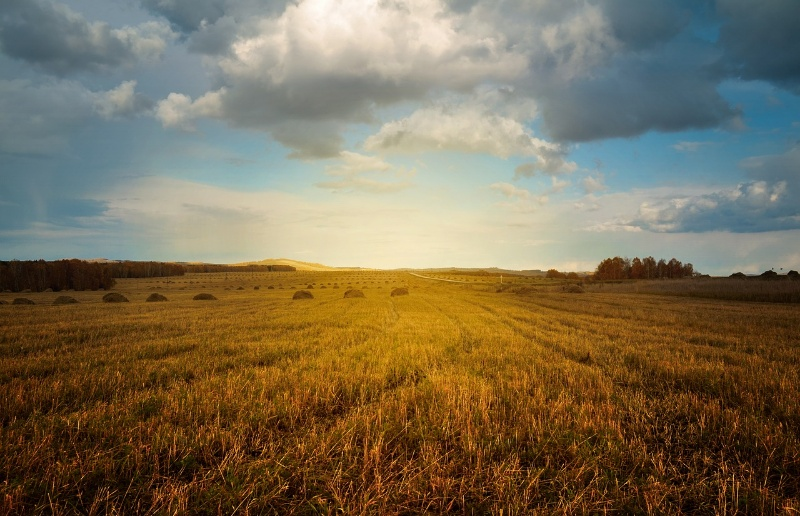
\includegraphics[scale=0.4]{parcelle2.jpg}
\caption{Une parcelle}
\end{figure}


Le terme de parcelle peut s'appliquer à différents domaine :

\begin{mylist}

\item En agriculture, elle désigne la division agricole (champ, pré, vignoble, verger, etc.) exploitée par la même personne ou le même groupe de personnes.


\item En urbanisme, elles sont définies selon leurs propriétaires et leurs limites, tant en milieu rural qu'urbain. Ainsi elle peut être un terrain habité, ou encore une parcelle à l'abandon ou bien une zone de stationnements automobiles. 

\end{mylist}



\subsection{La segmentation des parcelles}

La fragmentation spatiale des parcelles agricoles a un fort impact sur les flux d’eau dans les paysages cultivés, et pour surveiller les paysages à grandes échelles, il y a un fort besoin de délimitation automatique ou semi-automatique des parcelles agricoles. C’est pour cela que la contribution des images satellitaires à très haute résolution peut permettre la délimitation en utilisant de nombreuses méthodes de classification et des algorithmes qui traitent les caractéristiques de ces images.\cite{frag}

\begin{figure}[H]
\centering
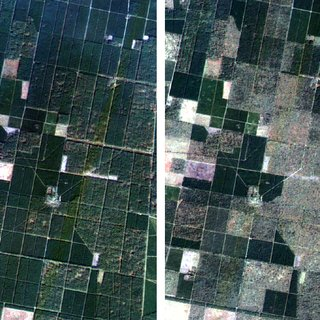
\includegraphics[scale=0.7]{seg.jpg}
\caption{La fragmentation d'une parcelle}
\end{figure}

Le résultat de ces études permet une bonne localisation des limites parcellaires et met en évidence l’intérêt d’un modèle global si une base de données d’images de limites parcellaires existe. 

\subsection{L'agriculture au Maroc}

L'agriculture est un secteur économique très important du Maroc. Il génère environ 14 \% du produit intérieur brut (PIB), mais avec des variations importantes (11 à 18 \%) selon les années en fonction des conditions climatiques. Ses performances conditionnent même celles de l’économie tout entière : le taux de croissance du pays est fortement corrélé à celui de la production agricole. L’agriculture demeure par ailleurs le premier pourvoyeur d’emplois du pays, loin devant les autres secteurs économiques, 40 \% de la population active vivant de ce secteur.\cite{imagesatt}

L’agro-industrie marocaine dont de nombreuses composantes jouissent de certifications ISO peut, légitimement être fière de tout le progrès accompli. Son savoir-faire confirmé lui permet de se placer sur de nombreux marchés extérieurs, très exigeants en qualité, avec des produits très diversifiés relevant de 10 classes différentes.\cite{agr}


\begin{figure}[H]
\centering
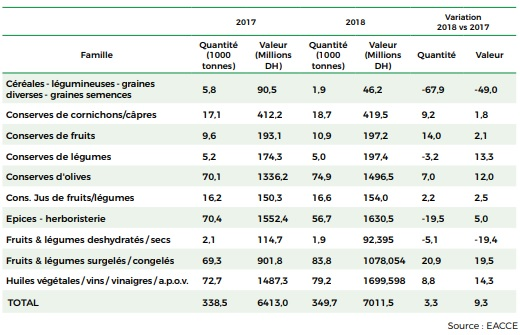
\includegraphics[scale=1.2]{agr.jpg}
\caption{L'agro-industrie au maroc entre 2017 et 2018}
\end{figure}


Les principales productions végétales du pays sont constituées par les céréales (blé, orge), les agrumes (oranges, clémentines), les olives, les rosacées fruitières (amandes, pommes, abricots...), les betteraves à sucre, les légumineuses alimentaires, les cultures maraichères dont les pommes de terre et les tomates, fer de lance des exportations agricoles marocaines. L'élevage (ovin, caprin, bovin, camelin, avicole) constitue aussi une composante importante du secteur agricole en contribuant à hauteur de 30 \% à sa valeur ajoutée.

\section{Les images satellites}

\subsection{Les sattelites en orbite autour de la terre}

Un satellite artificiel est un objet fabriqué par l'être humain, envoyé dans l'espace à l'aide d'un lanceur et gravitant autour d'une planète ou d'un satellite naturel comme la Lune.  
Le premier satellite artificiel Spoutnik 1 est lancé par l’Union des républiques socialistes soviétiques en 1957.
\par
Selon l'association UCS (Union of Concerned Scientists), 2.063 satellites opérationnels étaient en orbite autour de la Terre au 1er avril 2019. Le plus ancien encore en opération est un satellite amateur américain, Amsat-Oscar 7 (AO-7), lancé le 15 novembre 1974. La cadence des lancements s'est brusquement accélérée ces dernières années, avec 378 satellites lancés en 2017 et 375 satellites en 2018. Le 15 février 2017, l'Inde a ainsi battu un record avec 104 satellites en un seul tir.\cite{orbite}

\begin{figure}[H]
\centering
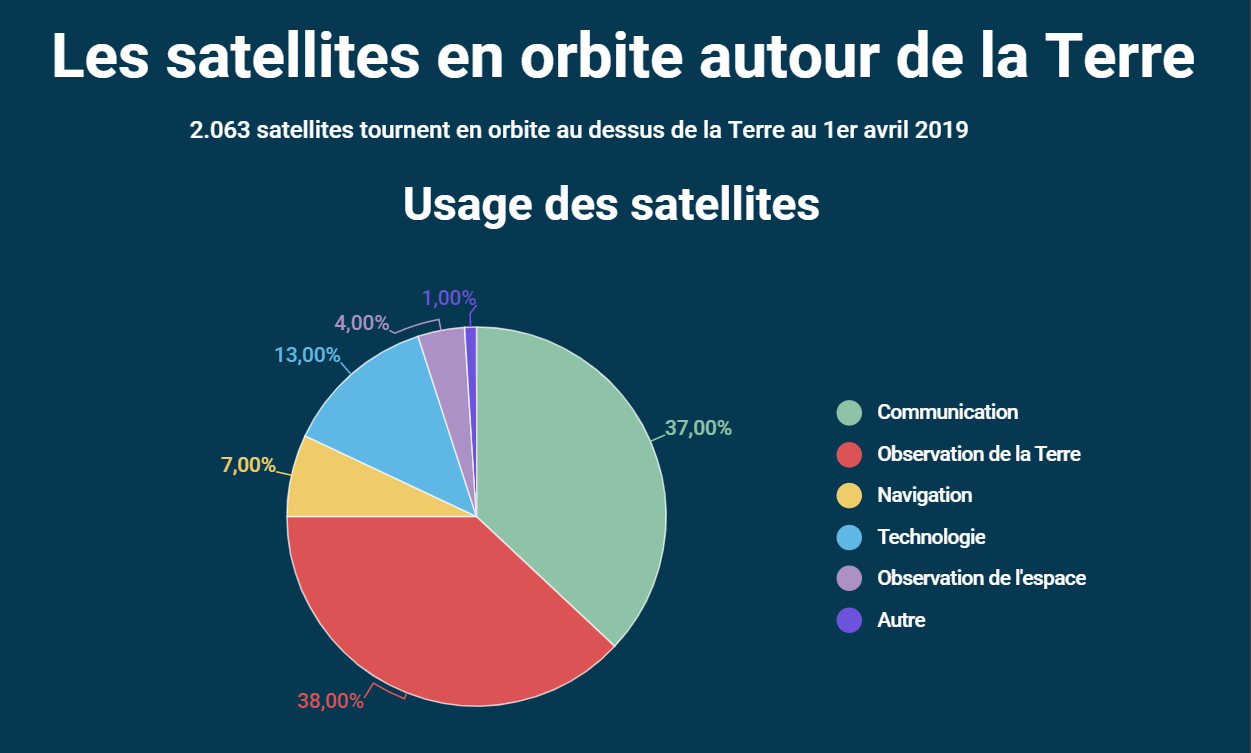
\includegraphics[scale=0.5]{satellite.png}
\caption{Statistiques de satellites}
\end{figure}

\subsection{Mission des sattelites Sentinels}
L'ESA (the European Space Agency) a developpé une nouvelle famille de mission pour sattelite appelé Sentinel dont le but d'une surveillance terrestre, océanique et atmosphérique en utilisant une gamme de technologie telles que le radar et les instruments d'imagerie multispectrale :
\begin{mylist}
\item \textbf{Sentinel-1} : est une mission d'imagerie radar en orbite polaire, tous temps, jour et nuit pour les services terrestres et océaniques;
\item \textbf{Sentinel-2} : est une mission d'imagerie haute résolution multispectrale en orbite polaire pour la surveillance des terres afin de fournir, par exemple, des images de la végétation, du sol et de la couverture hydrique, des voies navigables intérieures et des zones côtières;
\item \textbf{Sentinel-3} : est une mission multi-instruments pour mesurer la topographie de la surface de la mer, la température de la surface de la mer et de la terre, la couleur de l'océan et la couleur de la terre avec une précision et une fiabilité haut de gamme.\cite{sentinel}

\begin{figure}[H]
\centering
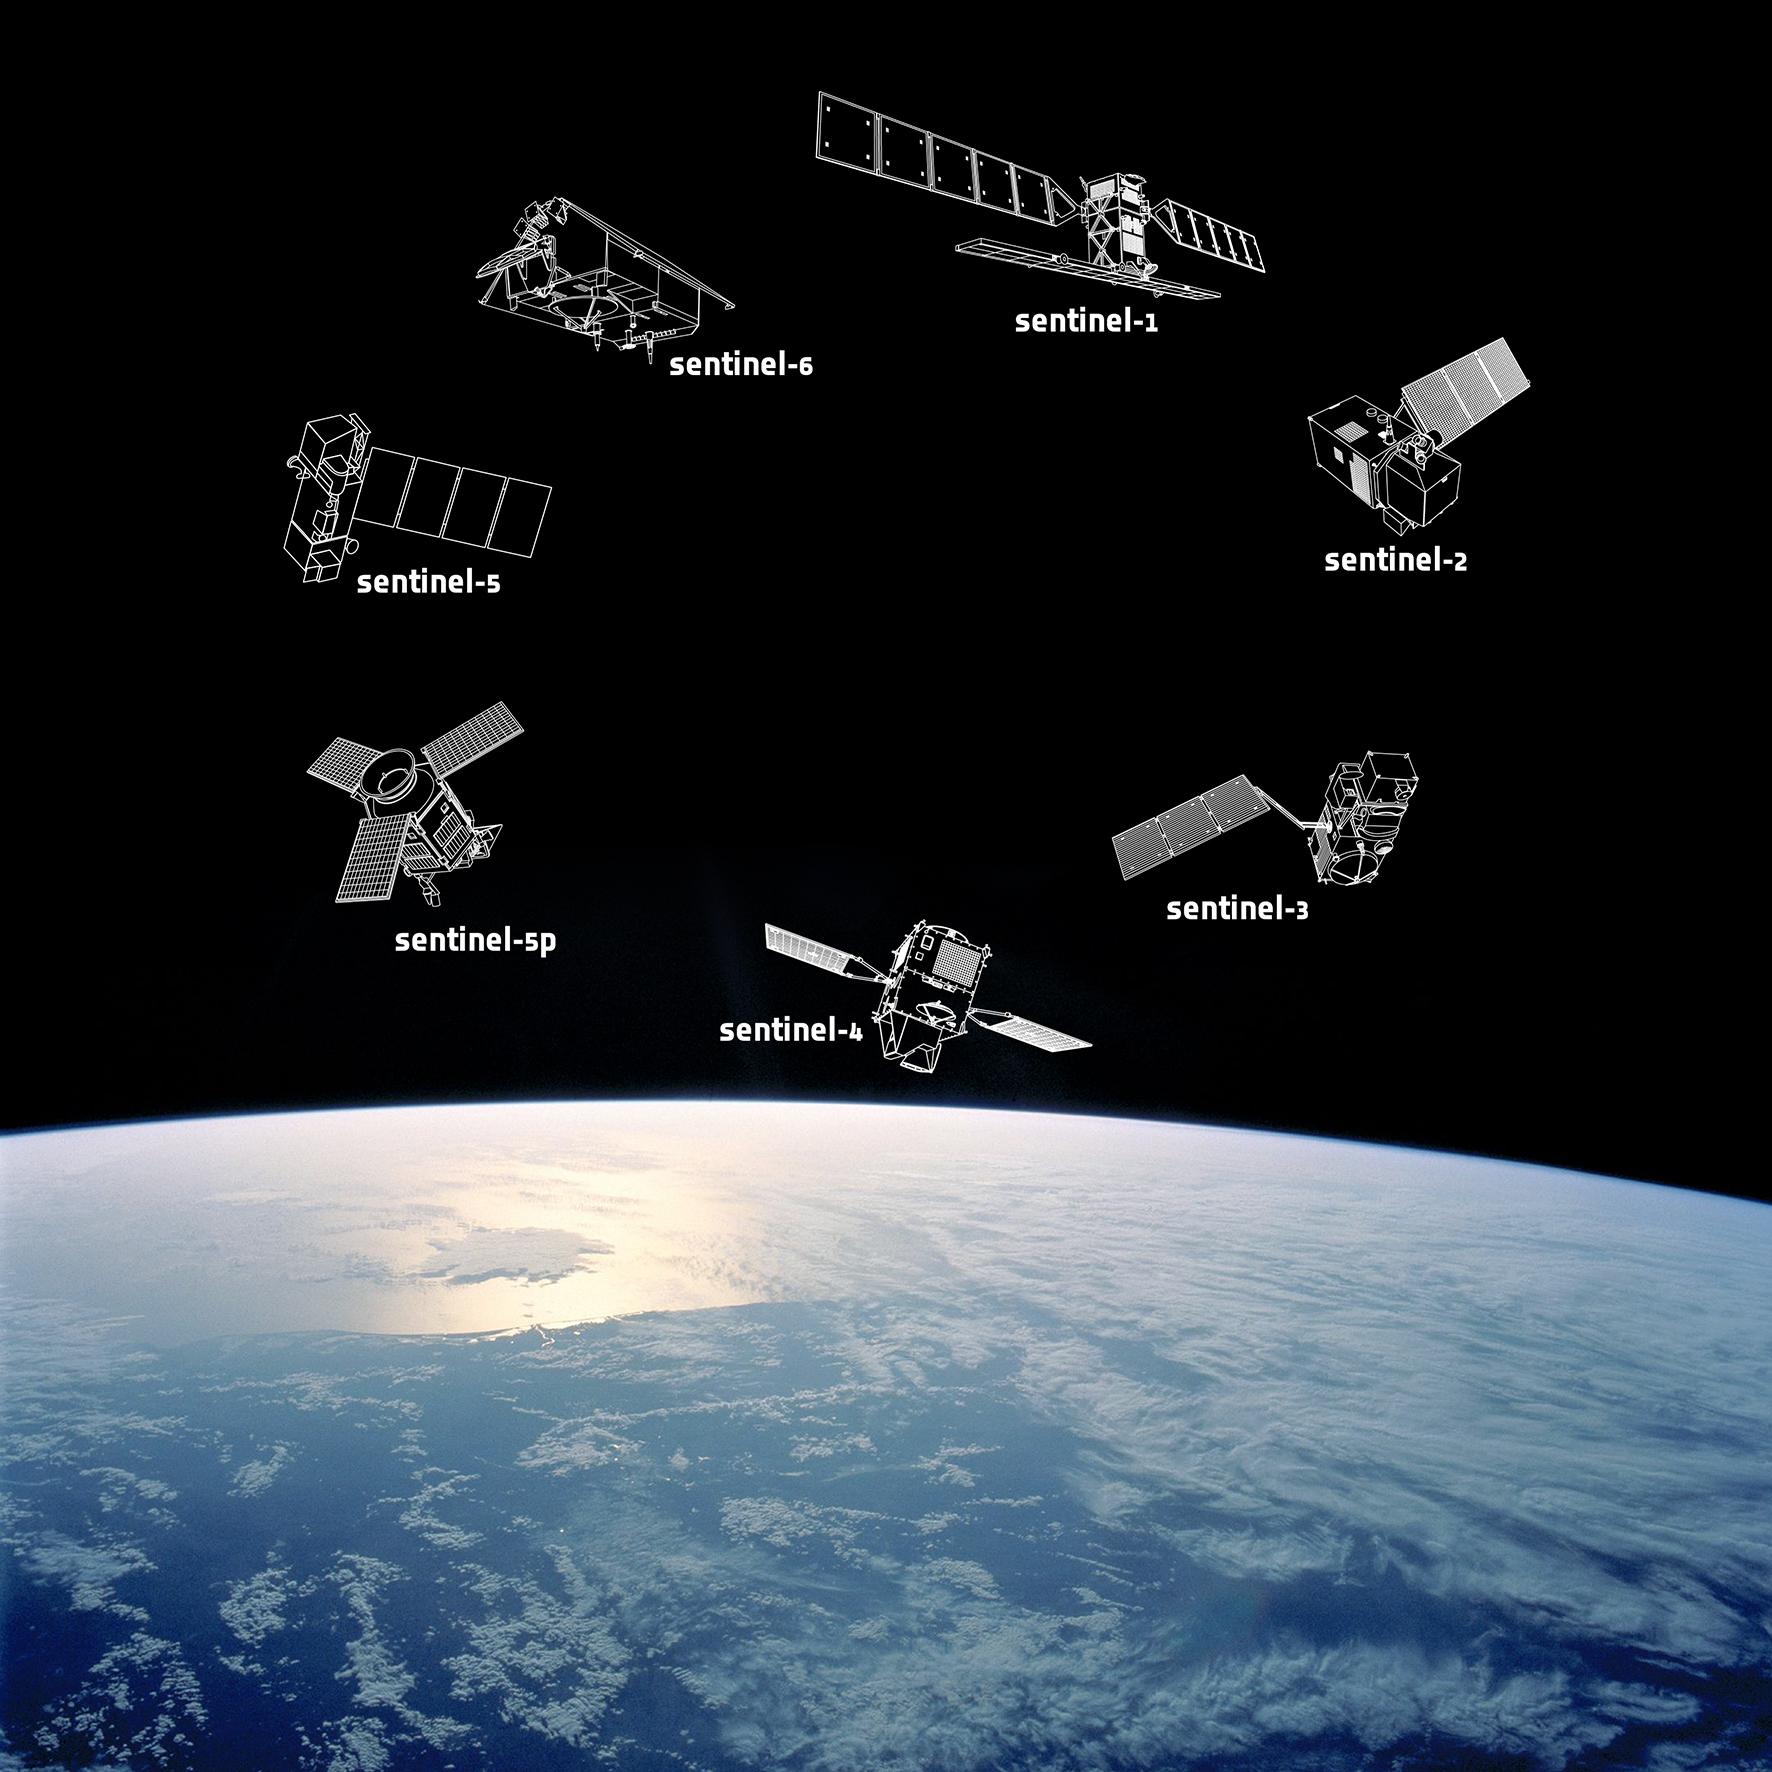
\includegraphics[scale=0.33]{Sentinel_family.jpg}
\caption{La famille des sattelites Sentinel}
\end{figure}

\end{mylist}

\subsection{Les satellites marocains}
Mohammed VI est un système de 2 satellites de reconnaissance et d'observation de la Terre (A et B) du type Pléiades, conçu par Thales Alenia Space (conception de la charge) et Airbus (conception de la plate-forme satellitaire) pour le compte du Centre royal de télédétection spatiale (Maroc).
\par
Le satellite Mohammed VI A est lancé le 8 novembre 2017 par un lanceur Vega depuis le Centre spatial de Kourou satellite espion, il est utilisé pour surveiller le Front Polisario dans la « zone tampon ».
Le lancement du deuxième satellite (Mohammed VI B) est effectué avec succès le 21 novembre 2018, à usage civil, est utilisé pour la cartographie et le cadastre, l’identification des zones sinistrées...
\begin{figure}[H]
\centering
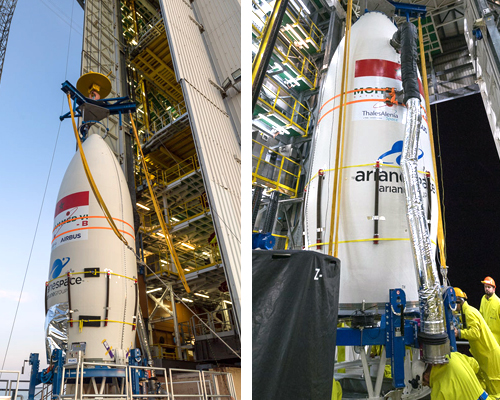
\includegraphics[scale=0.5]{satm6.jpg}
\caption{Le satellite MOHAMMED VI - B}
\end{figure}


\subsection{La définition d'une image satellite}
Une image satellite, ou image satellitaire, est une prise de vue transmise d'un satellite artificiel en orbite. Elles permettent d'obtenir différentes informations comme la surveillance des pays ennemis pour les militaires (fonction première de la création d'un satellite d'observation), prévisions météorologiques (par exemple les satellites Météosat), ou tout simplement pour les recherches sur l'Univers. Certains satellites sont capables d'une précision telle que cela peut devenir un problème, notamment en termes de vie privée ou de secret d'État. 

\subsection{Les caractéristiques des images satellites}
La principale différence entre une photographie et une image satellite est que la photographie est au format analogique et qu’elle est généralement imprimée sur papier avant d’être interprétée. L’image satellite est au format numérique et elle est généralement analysée et interprétée à l’aide d’un ordinateur.Le format numérique enregistre chaque bloc d’informations de manière discrète.


\par
\underline{Le pixel :}
\par

Avec un zoom avant suffisant sur une image satellite, on peut voir de nombreux carrés de couleurs différentes qui sont les pixels.
Ces pixels représente la plus petite unité figurant sur une image. Réunis, ils fournissent toute l’information qui constitue l’image dans son intégralité.

\par
\underline{La résolution spatiale :}
\par 

La résolution spatiale d’une image est la plus petite distance entre deux objets adjacents que le capteur puisse identifier.
Plus les pixels seront nombreux dans l’image plus la résolution spatiale sera élevée.
\par
Selon les caractéristiques du capteur, l’altitude du satellite ,son orbite autour de la Terre, les images satellites seront composées de pixels couvrant une surface plus ou moins grande du sol. On classera ainsi les images enregistrées en : Basse , moyenne, haute résolution ou très haute résolution.

\begin{figure}[H]
\centering
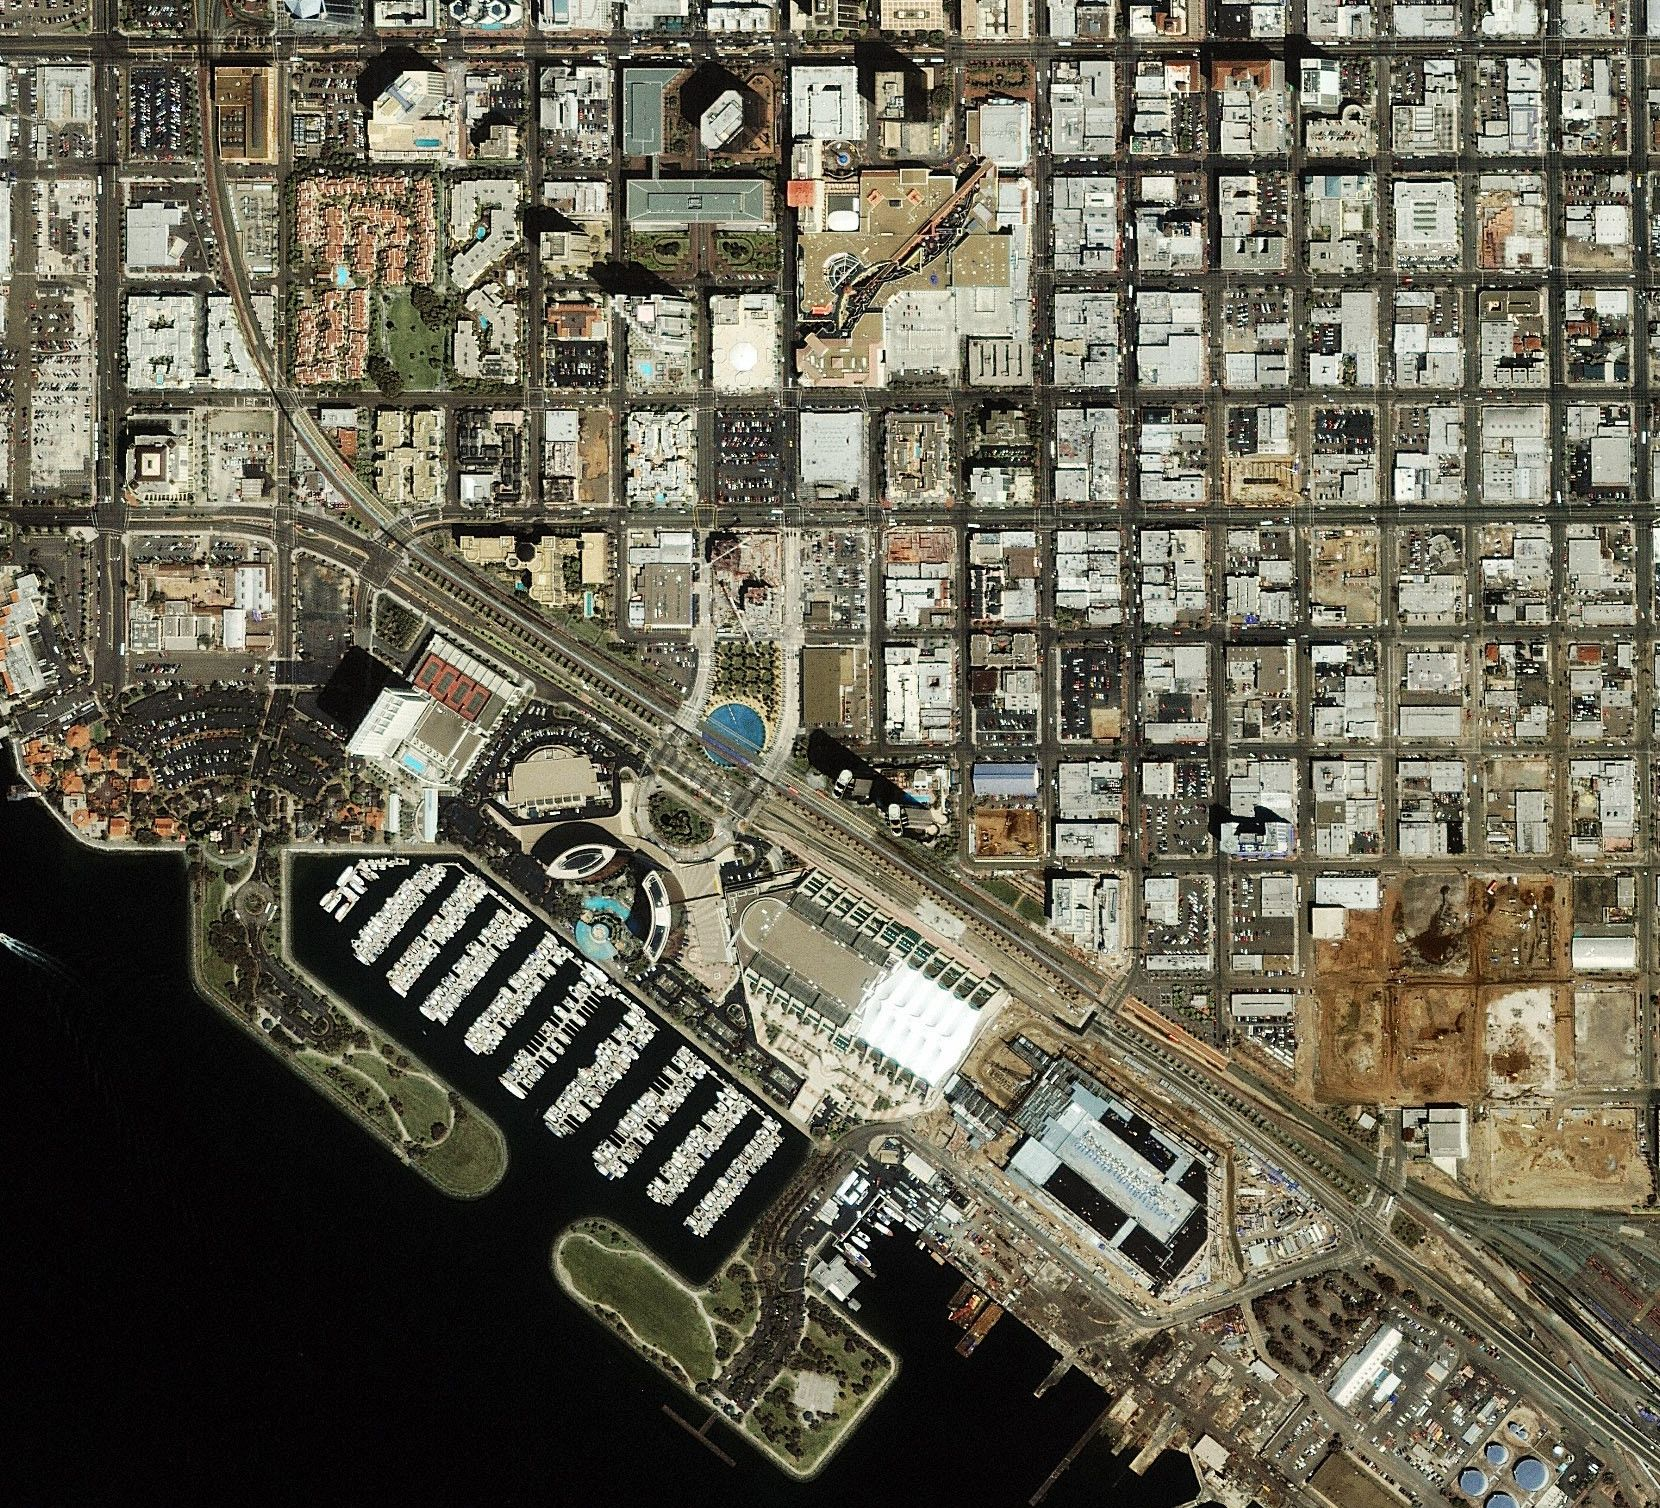
\includegraphics[scale=0.15]{resolution_image.jpg}
\caption{Image satellite en très haute résolution}
\end{figure}

\par
\underline{Valeur des pixels :}
\par 

Chaque pixel d’une image a une valeur. Cette valeur correspond à l’intensité du rayonnement réfléchi par l’objet observé dans la gamme de longueur d’ondes auxquelles le capteur est sensible. \cite{ref3}

La valeur du pixel varie de 0 (= noir) à 255 (= blanc). Donc, il y a 256 possibilités, ce qui correspond à 1 octet. Cela représente la quantité de rayonnement détectée par un capteur, allant du minimum au maximum. Le nombre de niveaux donne une indication quant à la précision de la mesure : plus il y a de niveaux (donc plus il y a de bits), plus détaillée sera la mesure et donc plus précise sera la mesure de la variation du rayonnement.

\begin{figure}[H]
\centering
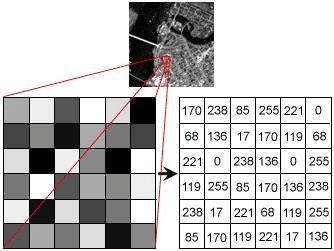
\includegraphics[scale=0.75]{pixel_values.png}
\caption{Les valeurs des pixels}
\end{figure}

\par
En observation de la Terre on peut exploiter :
\begin{mylist}
\item
des ondes émises par le soleil puis réfléchies par la surface de la Terre et enregistrées par un capteur placé sur un satellite.
\item
des ondes émises par un émetteur artificiel placé sur le satellite puis réfléchies par la surface de la Terre et enregistrées par un capteur placé sur ce même satellite.
\end{mylist}

Dans le premier cas on parle d'\textbf{images optiques} (télédétection passive), dans le second cas d'\textbf{images radar} (télédétection active).

\begin{figure}[H]
\centering
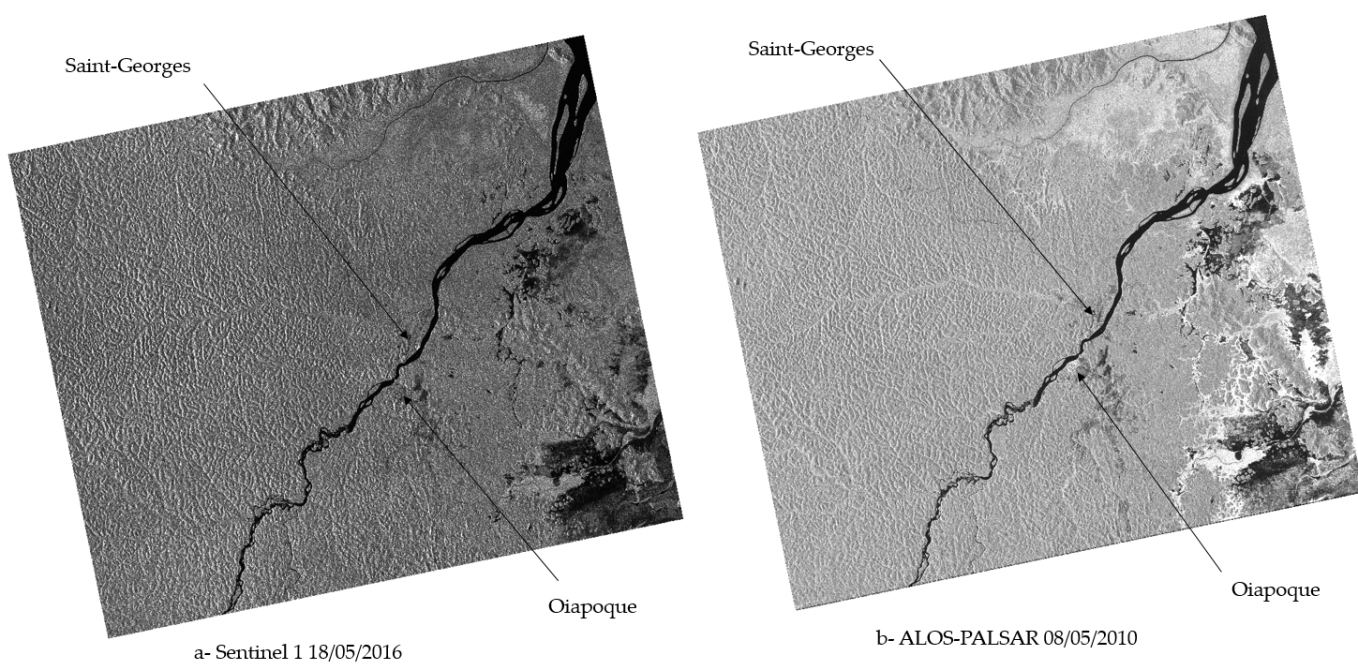
\includegraphics[scale=0.3]{image_radar.png}
\caption{Exemple d'image radar prise par le sattellite Sentinel-1 et ALOS/PALSAR}
\end{figure}

\par
La télédétection radar présente l’avantage de s’affranchir des contraintes de couverture nuageuse : les ondes émises par les satellites traversent les nuages pouvoir acquérir des images de jour comme de nuit. En revanche, leur exploitation pour l’observation de la Terre est moins intuitive quel les images optique, ainsi différents domaines spectraux sont exploité (longueurs d’onde du visible à l’infrarouge).\cite{ref4}



\subsection{Les satellites au service de l'agriculture}

Dans le domaine de l'agriculture, les satellites d'observation de la Terre sont utilisés pour une très grande variété d’applications et de services, comme la surveillance des cultures, le contrôle des surfaces et de l'occupation des sols, l'irrigation et la des gestion des cultures en engrais et produits phytosanitaires. Ils sont également utilisés pour suivre la production d'herbe tout au long de la saison culturale.  \cite{satt}


\begin{figure}[H]
\centering
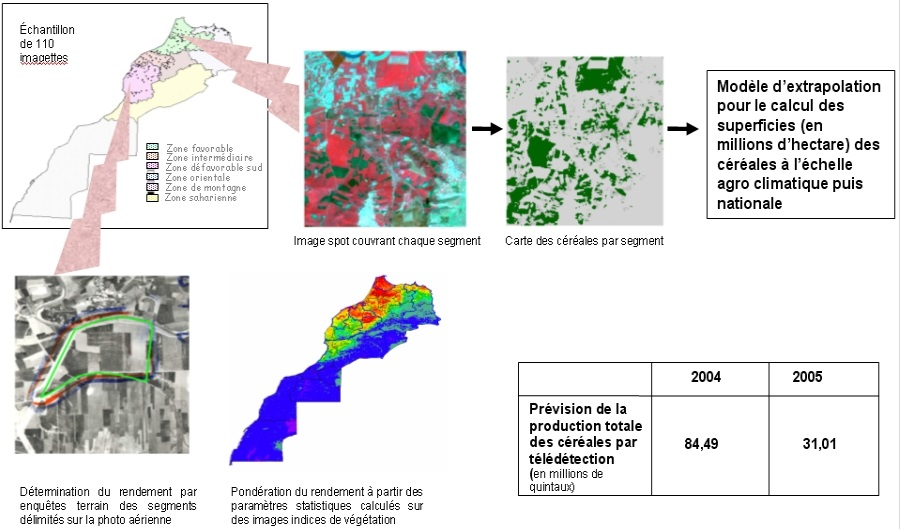
\includegraphics[scale=0.7]{prev.jpg}
\caption{Prévision de la production des céréales à l'échelle nationale}
\end{figure}

L'intérêt d'utiliser des satellites s'explique par leur capacité à  fournir des images multi spectrales de très bonne résolution. Ces images reçues dans plusieurs longueurs d'onde permettent d'estimer des paramètres biophysiques à partir des pixels de l'image que l'on mesure dans plusieurs couleurs de façon à caractériser l'état de la plante.\\
Les données des satellites sont utiles aux agriculteurs pour :
\begin{mylist}
\item dresser un portrait des caractéristiques et de la santé des sols et des cultures;
\item surveiller la croissance des pousses;

\item évaluer le taux d'humidité des sols et les besoins en irrigation;
\item estimer la production agricole totale.
\end{mylist}



\chapter{Analyse du sujet}


Ce chapitre abordera une analyse du sujet pour présenter le Crop Mapping et ses différentes méthodes en tant que technique qui permet la classification des parcelles en distinguant les différentes cultures, ainsi que des outils qu’on a pu tester pour faire la segmentation des images satellites. 

\newpage
\section{Crop Mapping}
\subsection{Définition}
C’est une technique en agriculture qui utilise des données GPS pour analyser des variables telles que le rendement des cultures et la teneur en eau dans un champ donné. Il a été développé dans les années 1990 et utilise une combinaison de technologie GPS et de capteurs physiques, tels que des compteurs de vitesse , pour suivre les rendements des cultures, la vitesse de l'élévateur à grains et combiner la vitesse.
\par
Ces données produisent une carte des rendements qui peut être utilisée pour comparer la distribution des rendements dans le champ d'une année à l'autre. Cela permet aux agriculteurs de déterminer les zones du champ qui, par exemple, peuvent avoir besoin d'être plus fortement irriguées ou qui ne produisent aucune récolte. Il permet également aux agriculteurs de montrer les effets d'un changement dans les techniques de gestion des champs, d'élaborer des stratégies nutritionnelles pour leurs champs et d'enregistrer le rendement des cultures à utiliser pour obtenir des prêts ou des locataires.

\subsection{Les méthodes de Crop Mapping}

\subsubsection{La télédétection (remote sensing from space)}

La télédétection offre une méthode sûre et efficace de cueillette d'information dans le but de cartographier le type et de calculer la superficie des cultures.
Les micro-ondes sont sensibles à l'alignement, la structure et la quantité d'eau présente dans les plantes et dans le sol, et peuvent fournir de l'information complémentaire aux données optiques. 

\par
La télédétection utilisant des satellites s'est révélée être un outil précieux pour une cartographie précise des cultures à travers le monde. La façon la plus conventionnelle d'effectuer des classifications de cultures par satellite est basée sur des observations multi-temporelles. Ils se sont révélés plus efficaces qu'une simple observation dans la classification des champs agricoles en raison de leur capacité à capturer plusieurs stades de croissance et différents types de structure des cultures, permettant une meilleure différenciation entre les cultures individuelles. \cite{cropmapp}

\begin{figure}[H]
\centering
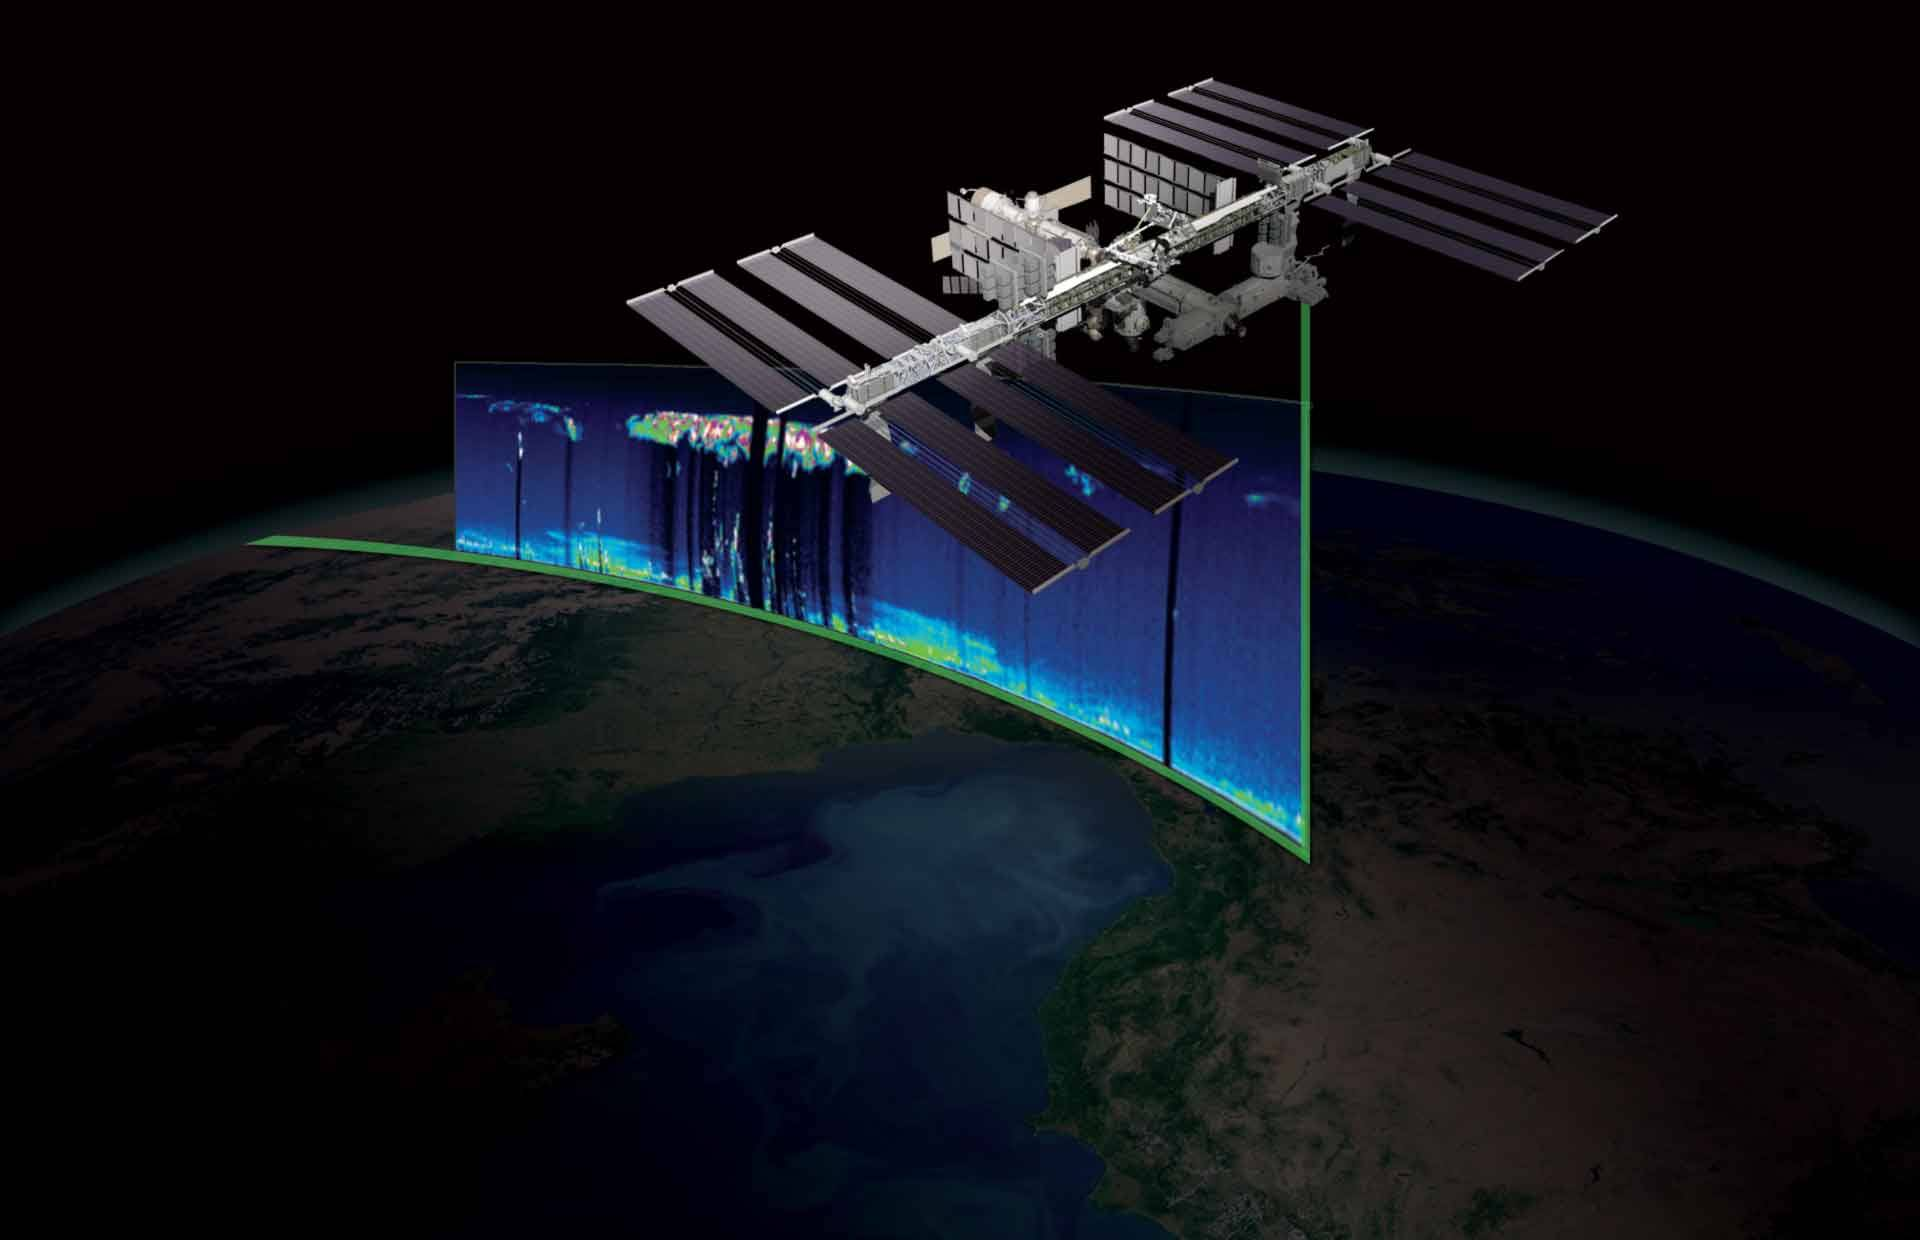
\includegraphics[scale=0.15]{tele.jpg}
\caption{La télédétection par satellite}
\end{figure}

\subsubsection{Utilisation de l'indice NDVI et de cartes satellites}

Il existe des modèles de surveillance directe sont utilisés pour analyser l'état des cultures sur la base des indices de télédétection directe fournis tels que l'indice de végétation par différence normalisée (NDVI). Habituellement, ces modèles sont faciles à adopter car ils nécessitent moins de données.

Les cartes NDVI sont utilisées dans la collecte d'informations sur la variabilité de la santé des cultures; identification des zones possibles où les cultures sont pauvres; établir le statut de développement des cultures; détecter les zones problématiques afin de prendre des décisions. Ces cartes sont utiles en ce qu'elles indiquent clairement les différences de croissance de la végétation dans une zone donnée. Habituellement, les valeurs NDVI ont une forte corrélation en ce qui concerne les stades de croissance des cultures et, par conséquent, c'est un moyen idéal pour déterminer la santé des cultures au cours de la période de croissance.

NDVI a un certain nombre d'applications, notamment la surveillance des cultures, des applications à taux variable, l'estimation du rendement et le dépistage. Souvent, des cartes de dépistage sont utilisées pour guider les agriculteurs sur les variations du champ afin de prendre la décision appropriée sur les mesures préventives et correctives à adopter. La surveillance des cultures, d'autre part, utilise des cartes NDVI pour surveiller la croissance des cultures dans le but de détecter toute anomalie au cours de la saison des cultures.

\begin{figure}[H]
\centering
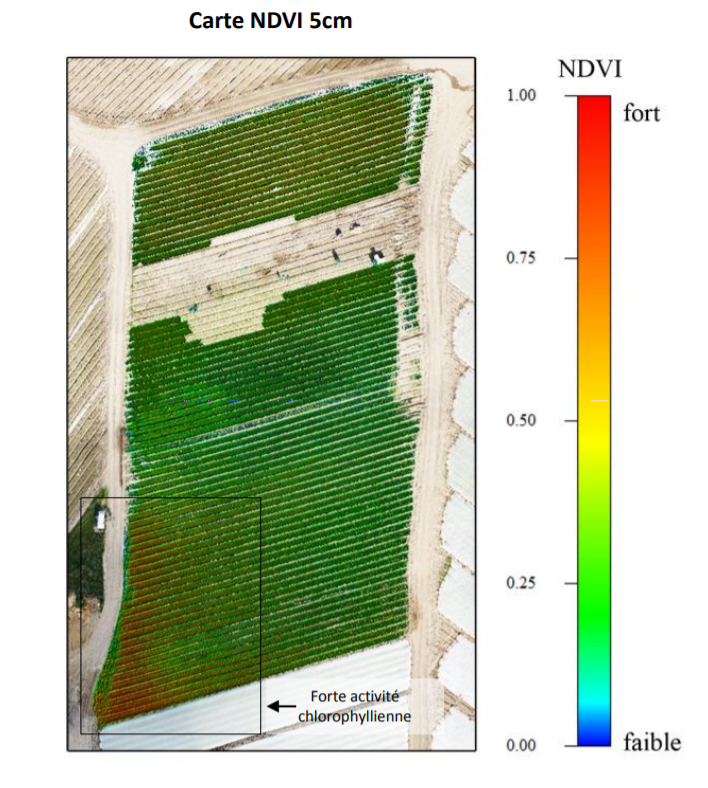
\includegraphics[scale=0.7]{ndvi.png}
\caption{L'indice NDVI}
\end{figure}



\subsubsection{Deep Learning Classification}
Le Deep Learning (DL) est une technique de pointe puissante pour le traitement d'image, y compris les images de télédétection (remote sensing images). 
Pour cibler la couverture des sols et la classification des types de cultures à partir d'images satellites multi-temporelles et multi-sources, une architecture DL à plusieurs niveaux solide doit être disposer. 
Le pilier de cette architecture est un réseau neuronal qui est utilisé pour la segmentation des images optiques et la restauration des données manquantes en raison des nuages et des ombres. \cite{deeplearning}

L’avantage de cette méthode est d’étudier des modèles de deep learning/machine learning pour la « crop classification » qui fournissent une segmentation basée sur les pixels d'une zone d'inspection pendant une période donnée. Pour obtenir de meilleurs résultats, il est préférable d’utiliser des modèles existant et de sélectionner ceux les mieux adaptés à la situation. Et pour mieux de flexibilité, il faut ajuster les modèles pré-formés par transfert learning à de nouvelles données comme de nouveaux domaines avec de nouvelles particularités, cultures...

Un autre avantage est le potentiel d'améliorer considérablement la précision d'un modèle avec plus de données réelles recueillies au sol de la région étudié en utilisant des données spécifiques. Cependant, il est possible d'obtenir de meilleurs résultats avec l'ensemble de données de formation (training data set) plus spécifiques.

\begin{figure}[H]
\centering
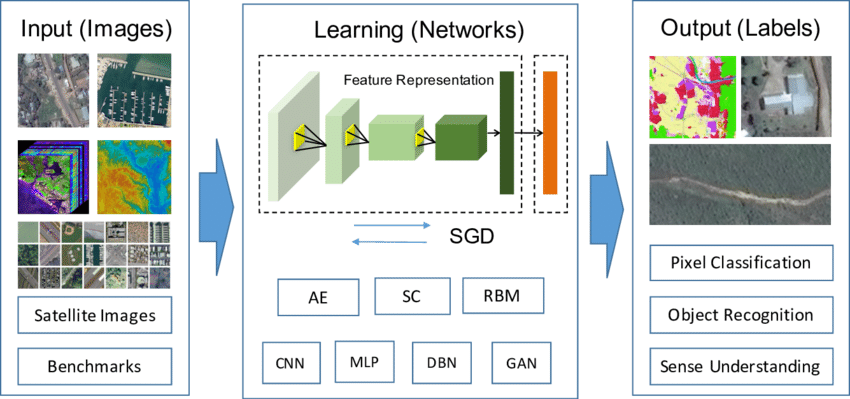
\includegraphics[scale=0.5]{deep.png}
\caption{Le processus de Deep Learning}
\end{figure}

\subsection{Outils pour le Crop Mapping}

On a essayé de faire une comparaison entre les outils les plus populaires dans le domaine du Crop Mapping :

{\setlength{\tabulinesep}{3pt}
\begin{tabu}{|c|c|c|c|c|c|c|}
\hline
\diagbox{caractéristiques}{L'outil}&\href{https://www.harrisgeospatial.com/Software-Technology/ENVI}{ENVI}&\href{https://qgis.org/fr/site/}{QGIS}&\href{https://www.arcgis.com/index.html}{ArcGIS}&\href{https://cmapsconnect.com/}{CMaps}&\href{https://clarklabs.org/terrset/}{TerrSet}&\href{https://groundwork.azavea.com/}{Groundwork}\\
\hline
Open Source & - & + & - & - & - & -\\
\hline
Imagerie 3D & - & + & + & - & - & -\\
\hline
Géocodage & - & + & + & + & + & -\\
\hline
Exportation d'images & + & + & + & - & + & +\\
\hline
Internet Mapping & + & - & + & + & - & -\\
\hline
L'interopérabilité & - & + & + & + & - & -\\
\hline
Étiquetage & + & + & + & - & - & +\\
\hline
Création de carte & + & + & + & + & + & +\\
\hline
Partage de carte & - & - & + & + & - & -\\
\hline
\end{tabu}}\\


\subsubsection{Au niveau des algorithmes :}


ENVI incorpore de nombreux algorithmes de fusion d'images bien connus (HSV transformation/Gram-Schmidt Spectral Sharpening, PC Spectral Sharpening/...) entre autres transformations de bande (Veg. Index calculation/ Tasseled Cap Transformation/ ...). Le côté positif est le fait que vous pouvez facilement programmer ENVI avec IDL pour effectuer des travaux de traitement par lots (beaucoup de données) ou créer un programme IDL autonome pour une autre transformation non déjà incluse dans ENVI.

QGIS est principalement conçu pour fonctionner avec des données vectorielles de type GIS (Geographic Information System), il prend en charge de nombreux formats d'images raster (svg, jpg, png, tif, ...) via les bibliothèques open source GDAL et GRASS.

Enfin, il existe de nombreux codes spécifiques au format pour plusieurs langages (Python, C, Java, etc.) qui vous permettront de lire les données et d'appliquer les transformations nécessaires.

\subsubsection{Test de l'outil QGIS :}
QGIS utilise Orfeo ToolBox (OTB) qui est une bibliothèque d’algorithmes de traitement d’image. OTB est basée sur la bibliothèque de traitement d’images médicales et fournit des fonctionnalités dédiées aux traitements d’images de télédétection ou pour les images de haute résolution spatiale. Les algorithmes dédiés aux images de grandes résolutions optiques (Pleiades, SPOT, QuickBird, WorldView, Landsat, Ikonos), aux capteurs hyperspectraux sensors (Hyperion) ou aux radars à synthèse d’ouverture (TerraSarX, ERS, Palsar) sont disponibles.
\begin{figure}[H]
\centering
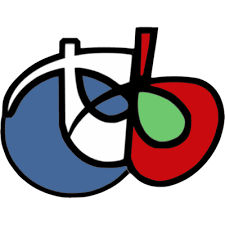
\includegraphics[scale=0.5]{orfeo.png}
\caption{La bibliothèque Orfeo ToolBox (OTB)}
\end{figure}

Le module "otb" permet l'utilisation de la bibliothèque de calcul numérique haute performance "TensorFlow" . L'API C ++ de TensorFlow est utilisée pour exécuter des sessions tensorflow à l' intérieur de filtres conformes au mécanisme de streaming d'ITK et OTB, ce qui signifie qu'il n'y a pas de limitation sur la taille des images à traiter.


Voici un exemple de segmentation qu'offre QGIS :
\begin{figure}[H]
\centering
\noindent
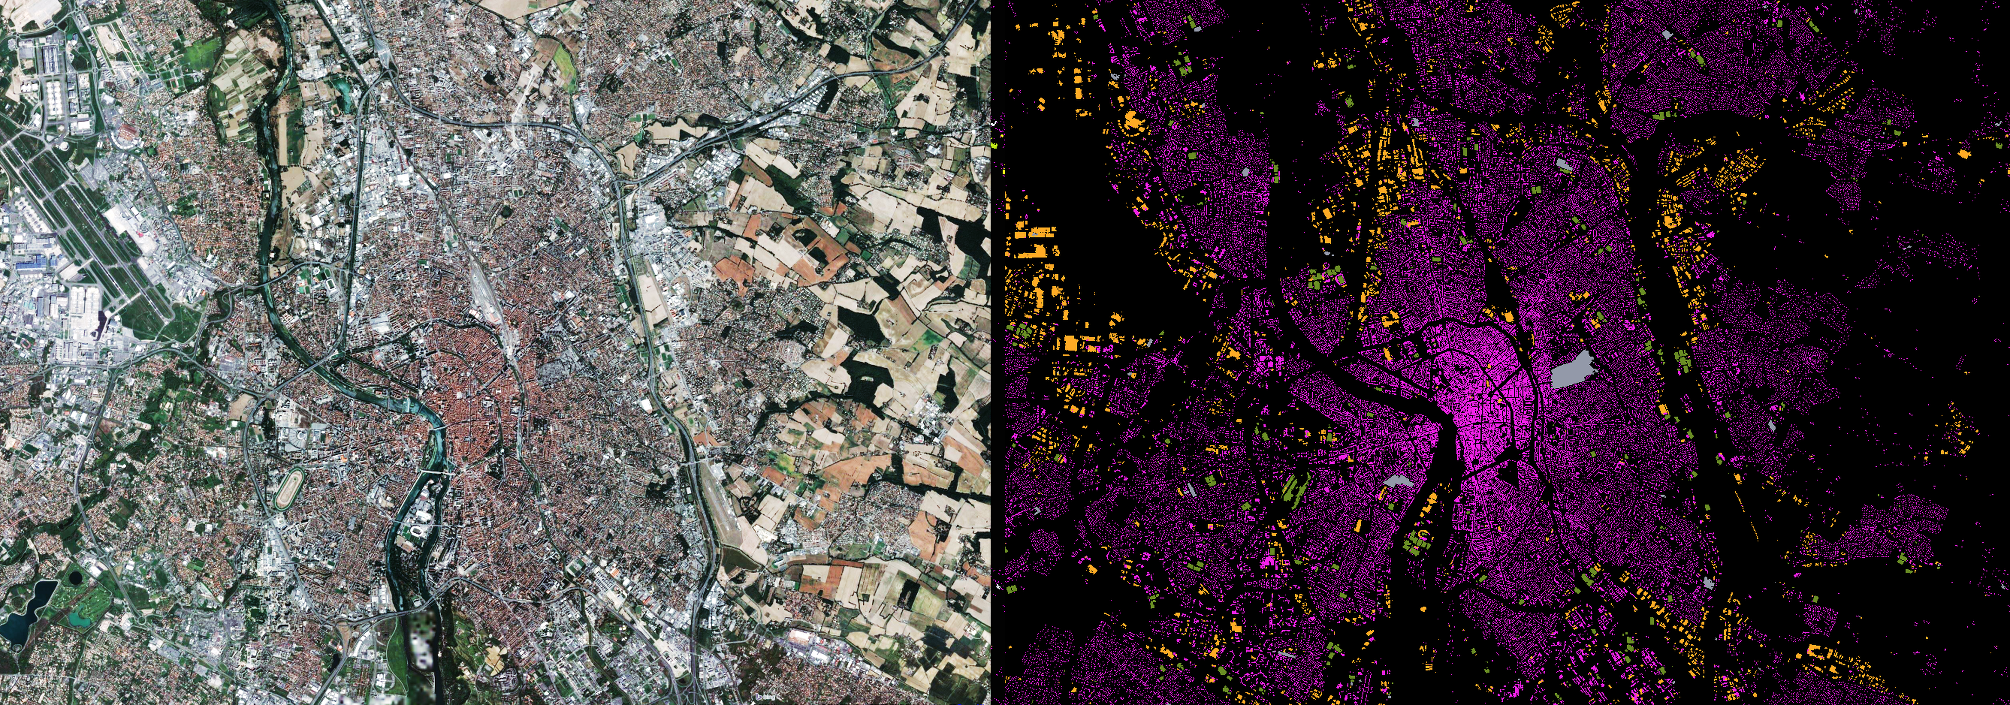
\includegraphics[width=1\textwidth]{test_segmentation.png}
\caption{Segmentation avec QGIS}
\end{figure}

\subsubsection{Test de l'outil Groundwork :}
\begin{figure}[H]
\centering

\includegraphics[scale=0.4]{Groundwork.png}
\caption{Groundwork logo}
\end{figure}

On a testé l'outil GroundWork de la compagnie azavea qui est en charge à la réalisation des modèles personalisé de machine learning qui analyse les images de drones et de satellites.
Cette outil qui est gratuit permet la création d'une "training data set" d'image géospatiale en implémentant une machine learning.
\par
La création du projet est comme ce qui suit : on determine d'abord le type du projet, c'est à dire soit détection d'objet, segmentation sémantique ou classification d'image, ensuite, on entre l'url de l'image qu'on veut ségmenter, puis on spécifie ce qu'on doit ségmenter (surface verte, l'eau, le sol ...) ainsi avec son processus de machine learning il nous ségmente notre image avec les classes que nous avons définis.
A la fin, on exporte notre image avec les étiquettes, mais aussi des données qu'on peut traiter avec pySTAC qui est une bibliothèque de python crée par la même compagnie.

\begin{figure}[H]
\centering
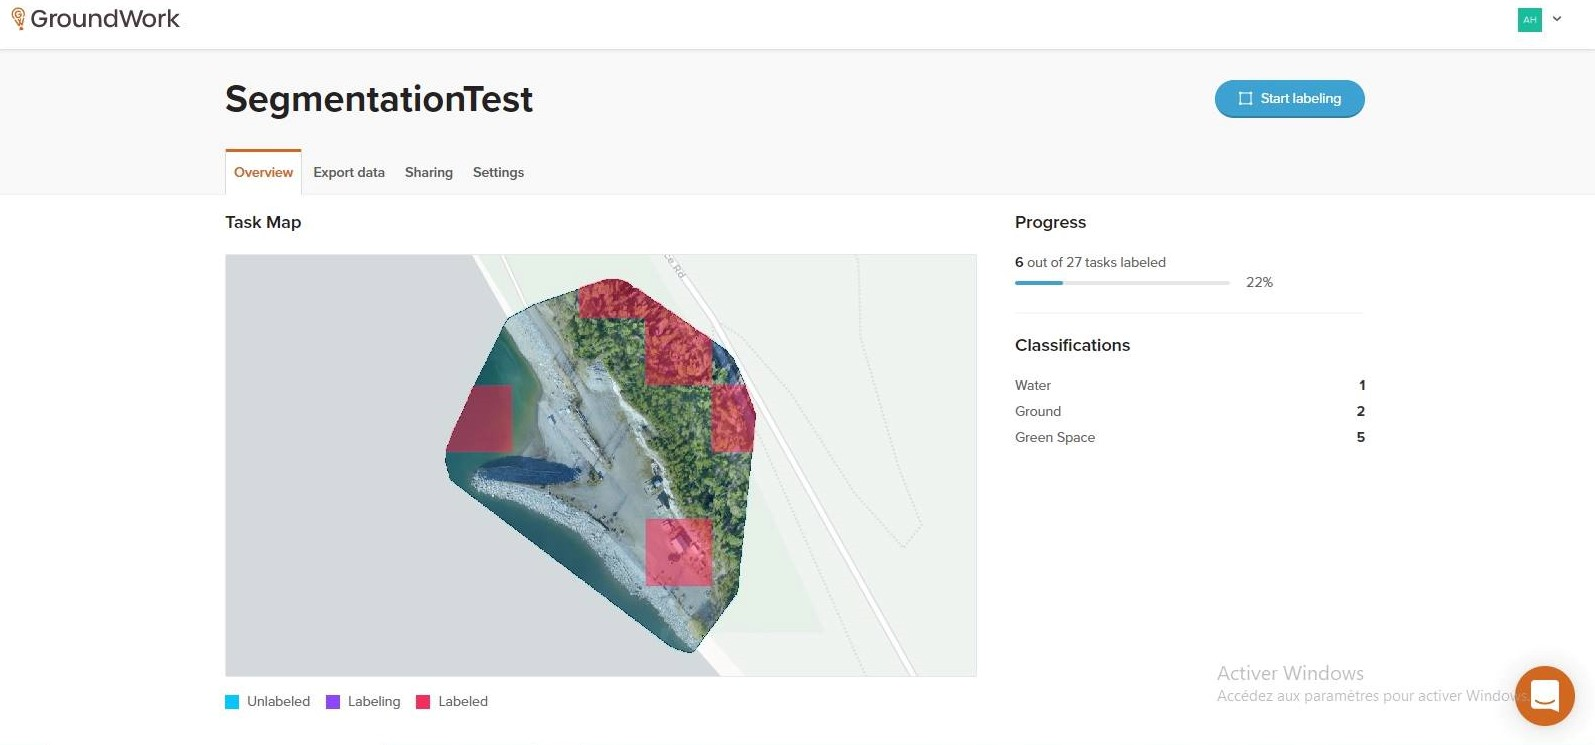
\includegraphics[scale=0.4]{groundwork_screen1.jpg}
\caption{Groundwork analysant l'image partie par partie}
\end{figure}

\begin{figure}[H]
\centering
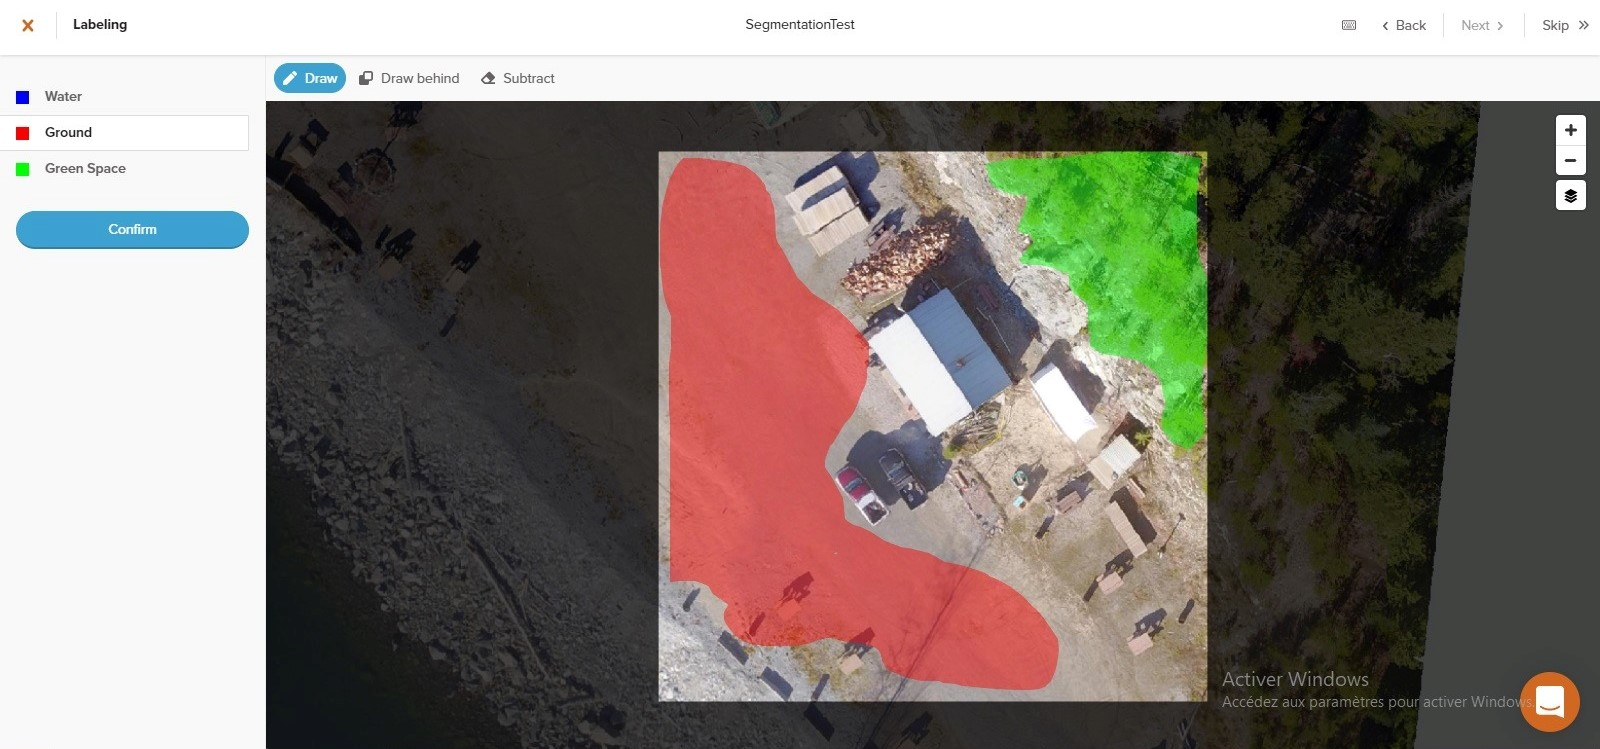
\includegraphics[scale=0.4]{groundwork_screen2.jpg}
\caption{Résultat d'une fragmentation d'un image avec des étiquettes}
\end{figure}

%Deuxième partie ____________________________________________________%

\chapter{Réalisation}

Le chapitre réalisation comporte les différents algorithmes qu'on a pu utiliser pour faire la segmentation des parcelles et aussi l'application de filtres qui permettent la détection des contours, et pour finir une comparaison des différents résultats qu'on a pu obtenir en appliquant le crop mapping à plusieurs images. 



\newpage

\section{Ségmentation et application des filtres}

\subsection{Algorithmes de segmentation}

\subsubsection{Support Vector Machine (SVM)}

\textbf{Définition :}\\
En Machine Learning, les machines à vecteurs de support (SVM) sont des modèles d'apprentissage supervisé avec des algorithmes d'apprentissage associés destinées à résoudre des problèmes de discrimination et de régression. 
\par
Un modèle SVM est une représentation des données sous forme de points dans l'espace, cartographiée de manière à ce que les données des catégories distinctes soient divisés par un espace clair aussi large que possible. De nouvelles données sont ensuite mappés dans ce même espace et devraient appartenir à une catégorie en fonction du côté de l'écart sur lequel elles se trouvent.
\begin{figure}[H]
\centering
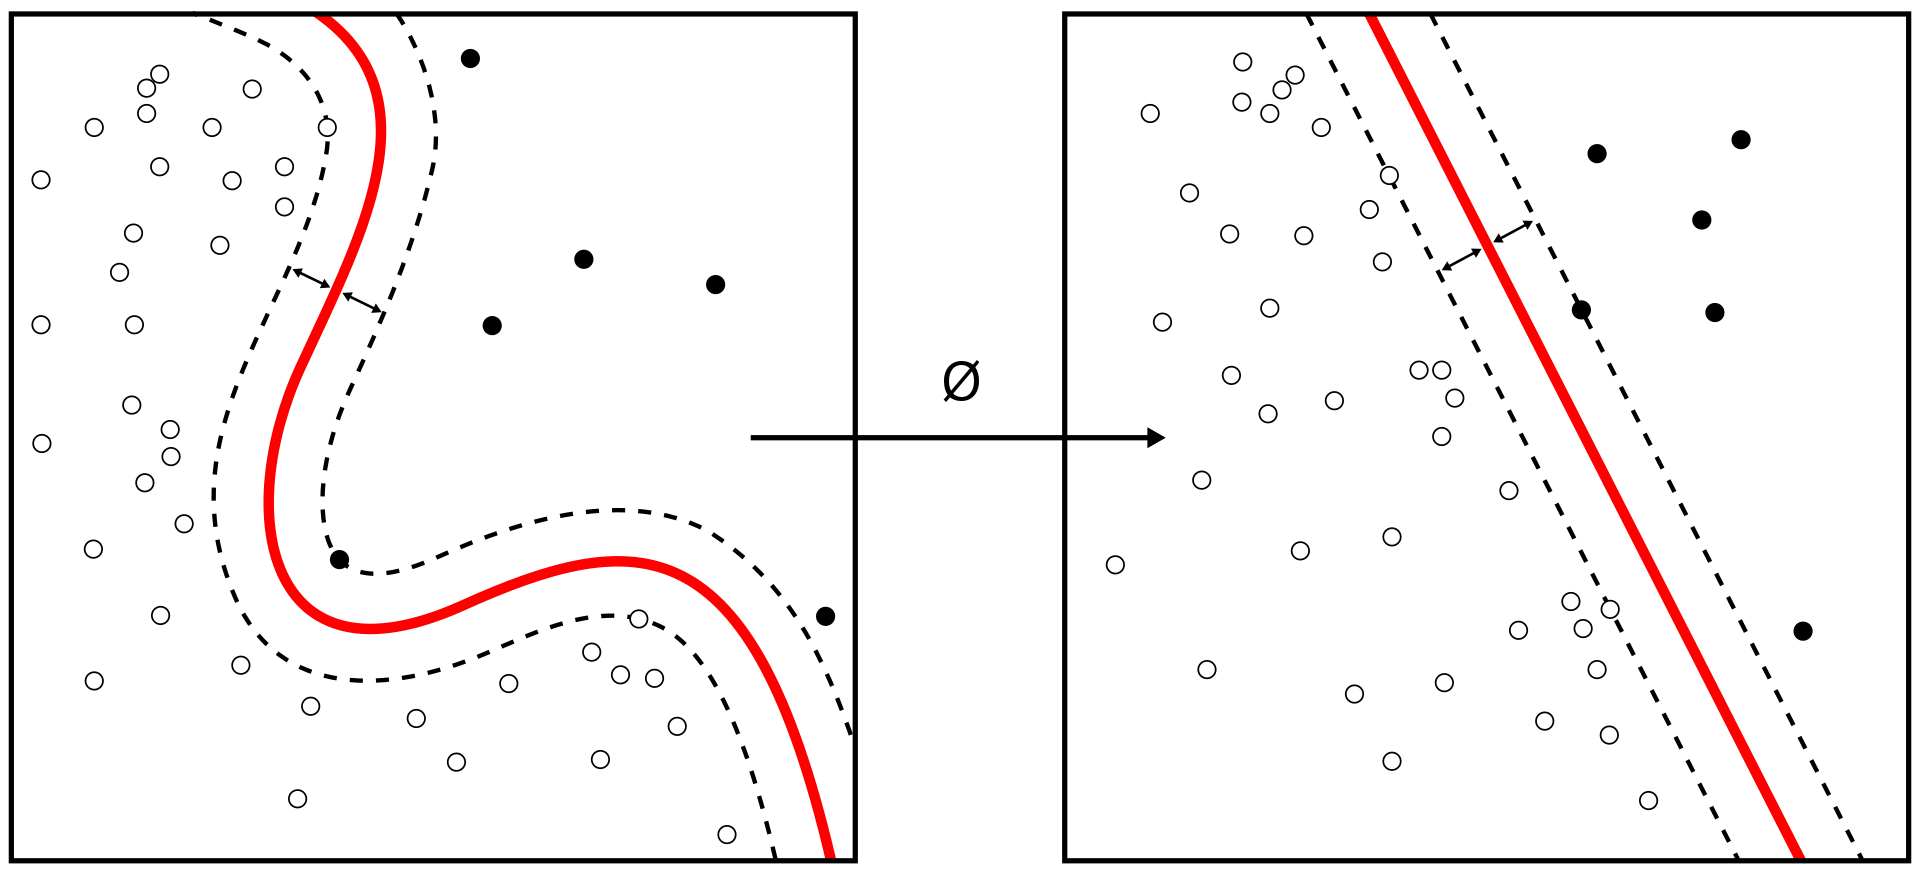
\includegraphics[scale=0.2]{svm.png}
\caption{Division de l'espace par SVM}
\end{figure}

\par
Les SVM ont été appliqués à de très nombreux domaines (bio-informatique, recherche d'information, vision par ordinateur, finance…). Selon les données, la performance des machines à vecteurs de support est de même ordre, ou même supérieure, à celle d'un réseau de neurones ou d'un modèle de mélanges gaussiens.

\textbf{SVM dans python :} \\
Dans Scikit-learn, les SVM sont implémentées dans le module "sklearn.svm".
Scikit-Learn contient la bibliothèque svm, qui contient des classes intégrées pour différents algorithmes SVM. 
\par
Nous avons effectuer une tâche de classification supervisé sur image sattelite d'une culture entre la région d'Assilah et Larache, nous utiliserons la classe de classificateur de vecteur de support, qui se nomme 'SVC' dans la bibliothèque svm de Scikit-Learn.
\par
Cette classe prend plusieurs paramètres qui sont en ralations avec des formules mathématiques correspondantes à SVM, et qui peuvent affecter le degré de netteté de la ségmentation.
\par
Voici un exemple d'une ségmentation en définissant trois classes sur l'image originale : 

\begin{figure}[H]
\centering
\hspace*{-0.5in}
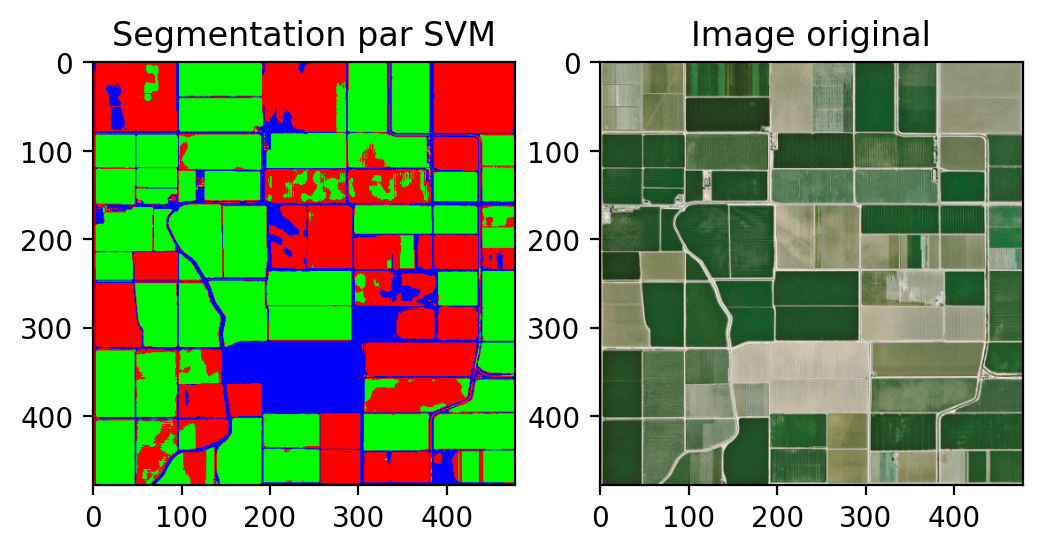
\includegraphics[scale=1.2]{classification.png}
\caption{Classification par SVM}
\end{figure}

\noindent Les classes sont les suivantes : 

\begin{mylist}
\item La partie verte : végétation.
\item La partie rouge : terre fertilisée.
\item La partie bleu : terre rocheuse.
\end{mylist}

\subsubsection{K-means algorithm}


\cite{k-means definition}K-means est un algorithme non supervisé de clustering non hiérarchique. Il permet de regrouper en K clusters distincts les observations du data set. Ainsi les données similaires se retrouveront  dans un même cluster. Par ailleurs, une observation ne peut se retrouver que dans un cluster à la fois (exclusivité d’appartenance). Une même observation, ne pourra donc, appartenir à deux clusters différents.



Pour pouvoir regrouper un jeu de données en K cluster distincts, l’algorithme K-Means a besoin d’un moyen de comparer le degré de similarité entre les différentes observations. Ainsi, deux données qui se ressemblent, auront une distance de dissimilarité  réduite, alors que deux objets différents auront une distance de séparation plus grande, cette distance sont calculé par des formules mathématiques et statistiques comme par exemple la distance euclidienne.

La determination du nombre de cluster K peut conduire à un partitionnement trop fragmenté des donnée si on a un jeu de données très grand. Par contre, un nombre de clusters trop petit, conduira à avoir des cluster trop généralistes contenant beaucoup de données.

La méthode la plus usuelle pour choisir le nombre de clusters est de lancer K-Means avec différentes valeurs de K et de calculer la variance des différents clusters.  La variance est la somme des distances entre chaque centre de cluster (centroid) et les différentes observations inclues dans le même cluster. 
\newline
\textbf{ La variance des clusters se calcule comme suit :\\}
\makebox[\textwidth]{
   $ V = \sum_{j} \sum_{x_i\rightarrow c_j} D(c_j,x_i)^2$
    }
    
Avec :
\begin{mylist}


\item $c_j$ : le centre du cluster (le centroid)
\item $x_i$: la ième observation dans le cluster ayant pour centroïd $c_j$
\item $D(c_j,x_i)$ : La distance (euclidienne ou autre) entre le centre du cluster et le point $x_i$
\end{mylist}


\textbf{\underline{Fonctionnement de l’algorithme K-Means}}\cite{k-means}

\begin{enumerate}
    %1-
    \item Donner en entrée K le nombre de cluster à former et Le Training Set (matrice de données)
        \begin{figure}[ht]
        \centering
        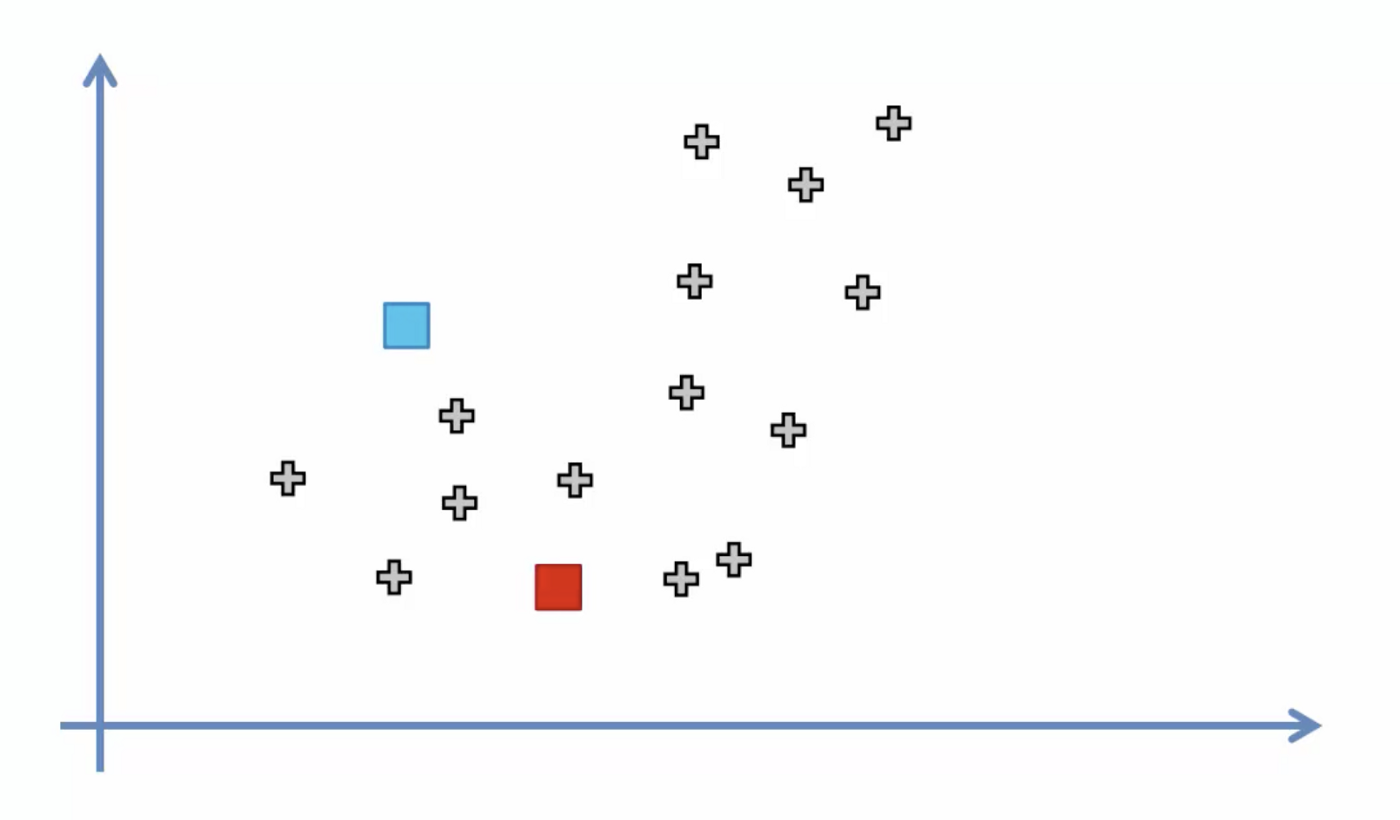
\includegraphics[scale=0.2]{algo1.png}
        \end{figure}
    %2-
    \item Attribuez chaque point de données au cluster le plus proche en calculant sa distance par rapport à chaque centroïde (centre du cluster)
        \begin{figure}[H]
        \centering
        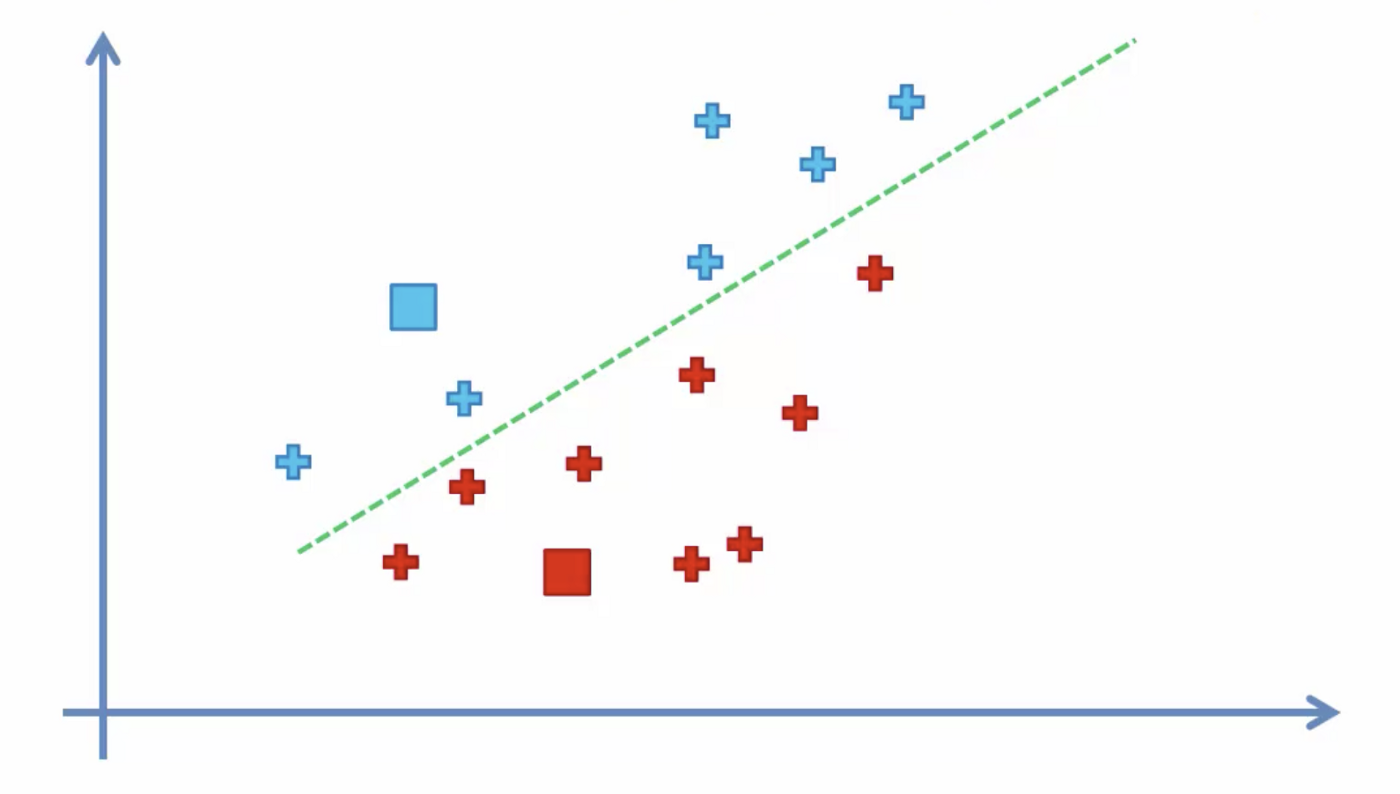
\includegraphics[scale=0.2]{algo2.png}
        \end{figure}
    %3-
    \item Déterminez le nouveau centre du cluster en calculant la moyenne des points attribués
        \begin{figure}[H]
        \centering
        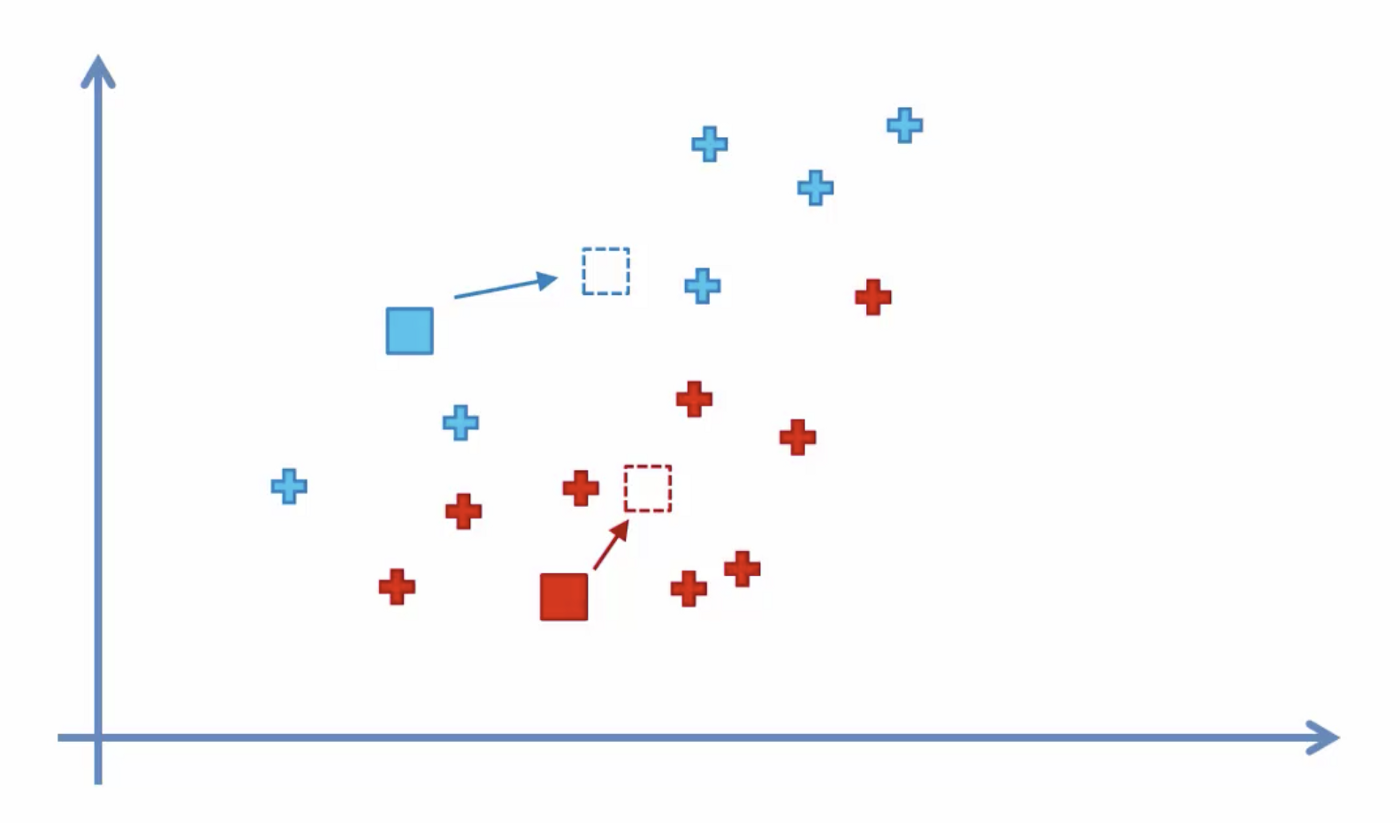
\includegraphics[scale=0.2]{algo3.png}
        \end{figure}
    %4-
    \item Répéter les étapes 2 et 3 jusqu'à ce qu'aucune des affectations de cluster ne change
        \begin{figure}[H]
        \centering
        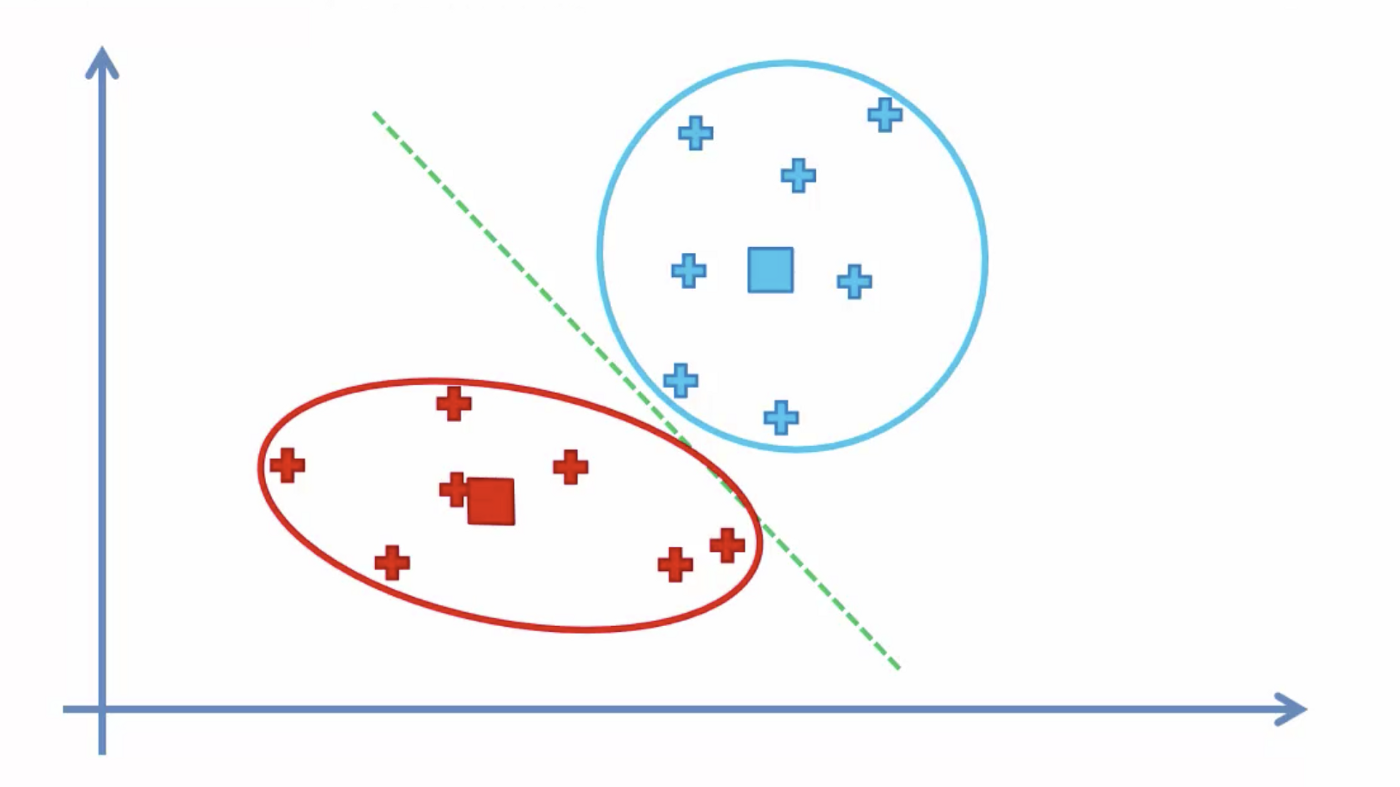
\includegraphics[scale=0.2]{algo4.png}
        \end{figure}
\end{enumerate}


\par
Pour son application on a utilisé la même image précédente et on a définie trois cluster pour la ségmentation voice le résultat : 

\begin{figure}[H]
\centering
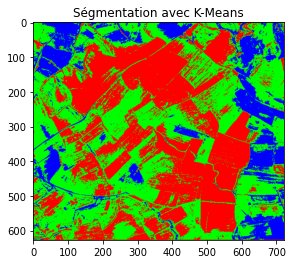
\includegraphics[scale=1.2]{kmeans.png}
\caption{Segmentation avec K-Means}
\end{figure}

\subsubsection{Multi-Otsu threshold}
\cite{otsu}Multi-Otsu Threasholding est un algorithme de seuillage utilisé pour séparer les pixels d'une image d'entrée en plusieurs classes différentes, chacune obtenue en fonction de l'intensité des niveaux de gris dans l'image.
Multi-Otsu calcule plusieurs seuils, déterminés par le nombre de classes (le nombre de classes par défaut est 3) en passant par toutes les valeurs de seuil possibles (de 0 à 255), le but est donc de trouver la valeur du seuil optimale de l'image d'entrée en calculant et en évaluant la variance inter-classe (ou variance intra-classe).

Les formules pour calculer les variances entre les classe pour la méthodes Otsu :

\makebox[\textwidth]{
   $ \sigma_\omega^2(t) = \omega_1(t)\sigma_1^2(t) + \omega_2(t)\sigma_2^2(t)$
    }
Avec : 
\begin{mylist}
\item $\omega_i$ : la probabilité d'être dans la $i$ème classe, , chacune étant séparée par un seuil $t$
\item $\sigma_i^2$ : les variances de ces classes
\end{mylist}

Otsu montre que minimiser la variance intra-classe revient à maximiser la variance inter-classe : 

\makebox[\textwidth]{
   $ \sigma_b^2(t) =  \sigma^2 - \sigma_\omega^2(t)=
   \omega_1(t)\omega_2(t)[\mu_1(t)-\mu_2(t)]^2$
    }
Avec $\mu_i$ la moyenne des classes

\textbf{\underline{Fonctionnement de l’algorithme Multi-Otsu threshold}}

\begin{enumerate}
    \item Calculer l'histogramme et les probabilités de chaque niveau d'intensité
    \item Définir les $\omega_i(0)$  et $\mu_i(0)$ initiaux
    \item Parcourir tous les seuils possibles $t=1,\ldots,n=$intensité max
    \begin{enumerate}
        \item Mettre à jour $\omega_{i}$ et  $\mu_{i}$
        \item Calculer $\sigma_{b}^{2}(t)$
    \end{enumerate}
    \item Le seuil désiré correspond au $\sigma_{b}^{2}(t)$ maximum.
\end{enumerate}



\begin{figure}[H]
\centering
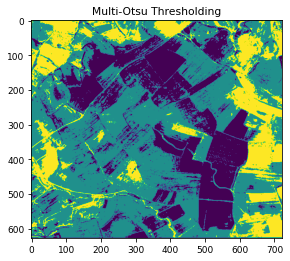
\includegraphics[scale=1.2]{osupng.png}
\caption{Segmentation avec multi-Otsu threshold}
\end{figure}

\subsection{Comparaison des méthodes de détection des contours}
Le contour c’est la zone où il existe des différences extrêmes dans les intensités du pixel indique généralement un bord d'un objet.
Nous mettrons en œuvre certaines des méthodes les plus utilisées et utiliserons également les méthodes d'Open CV et de PIL.\cite{comparaison}
\noindent Nous comparerons les méthodes suivantes:
\begin{mylist}
\item Détecteur de contour Sobel
\item Détecteur de contour Prewitt
\item Détecteur de contour Canny
\item Détecteur de contour Gabor
\end{mylist}

\subsubsection{Opérateur Sobel}
Sobel est un opérateur très courant pour détecter les bords d'une image, qui est une approximation d'une dérivée d'une image. Il est séparé dans les directions 'y' et 'x'. Ici, nous utilisons une matrice de noyau 3 * 3, une pour chaque direction 'x' et 'y'. Le gradient pour la direction 'x' a des nombres négatifs à gauche et des nombres positifs à droite et nous préservons les pixels centraux. De même, le gradient pour la direction 'y' a des nombres négatifs en bas et des nombres positifs en haut .

\begin{figure}[H]
\centering
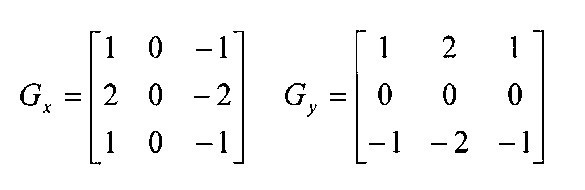
\includegraphics[scale=0.9]{sobel_masque.jpg}
\caption{Les masques de Sobel}
\end{figure}

Voici le résultat en appliquant le filtre de Sobel à l'image original :

\begin{figure}[H]
\centering
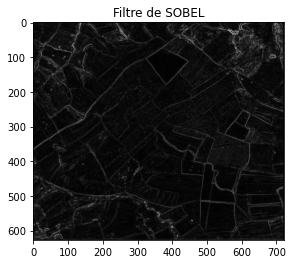
\includegraphics[scale=1.2]{sobel_result.png}
\caption{Filtre de Sobel appliqué à l'image originale}
\end{figure}


\subsubsection{Opérateur de Prewitt}
L'opérateur de Prewitt est similaire à l'opérateur de Sobel, il est utilisé pour détecter les contours verticaux et horizontaux dans les images. Cependant, contrairement au Sobel, cet opérateur ne met pas l'accent sur les pixels les plus proches du centre du masque.

\begin{figure}[H]
\centering
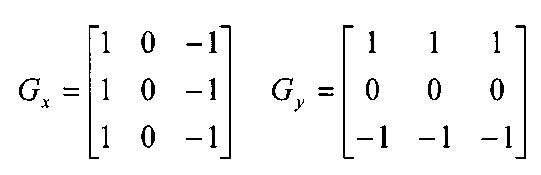
\includegraphics[scale=0.9]{prewit_masque.png}
\caption{Les masques de prewitt}
\end{figure}

Au niveau du code, la seule différence est le masque.
Le résultat est le suivant : 
\begin{figure}[H]
\centering
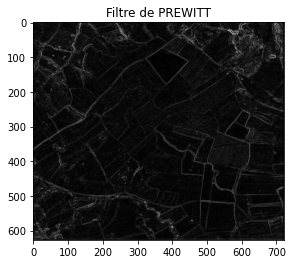
\includegraphics[scale=1.2]{prewitt_result.png}
\caption{Application du filtre de Prewitt}
\end{figure}

\subsubsection{Opérateur Canny}
Le détecteur de contour Canny est probablement la méthode la plus utilisée et la plus efficace, c'est une méthode de détection de contour beaucoup plus complexe que celles décrites ci-dessus.
\noindent Les étapes de cette méthode sont les suivantes :
\begin{enumerate}
    \item Lissage de l'image avec un filtre gaussien pour réduire le bruit.
    \item Le calcul du gradient en utilisant l'un des opérateurs de gradient Sobel ou Prewitt.
    \item Extraction des points de contour: suppression non maximale.
    \item Liaison et seuillage: hystérésis
\end{enumerate}

Après les deux premières étapes, il faut également calculer l'orientation des gradients «thêta = arctan (Gy / Gx)». Gy et Gx sont respectivement la direction x du gradient et la direction y.
Parlons maintenant de la suppression non maximale et de ce qu'elle fait. Dans cette étape, nous essayons de relier la direction des contours à une direction qui peut être tracée le long des contours en fonction des forces de gradient et des directions des contours précédemment calculées. À chaque emplacement de pixel, nous avons quatre directions possibles. Nous vérifions toutes les directions si le gradient est maximum à ce point. Les valeurs de pixels perpendiculaires sont comparées à la valeur dans la direction du contour. Si leur valeur est inférieure au pixel sur le contour, ils sont supprimés. Après cette étape, nous obtiendrons des contours minces cassés qui doivent être réparés, alors passons à l'étape suivante.
L'hystérésis est un moyen de relier les lignes brisées produites à l'étape précédente. Cela se fait en itérant sur les pixels et en vérifiant si le pixel actuel est un contour. S'il s'agit d'un contour, vérifiez les environs pour les contours. S'ils ont la même direction, nous les marquons comme pixel de contour. Nous utilisons également 2 seuils, un haut et un bas. Si les pixels sont supérieurs au seuil inférieur, ils sont marqués comme un contour. Ensuite, les pixels supérieurs au seuil inférieur et également supérieurs au seuil élevé sont également sélectionnés comme pixels à fort contour. Quand il n'y a plus de changements à l'image, nous nous arrêtons.

\begin{figure}[H]
\centering
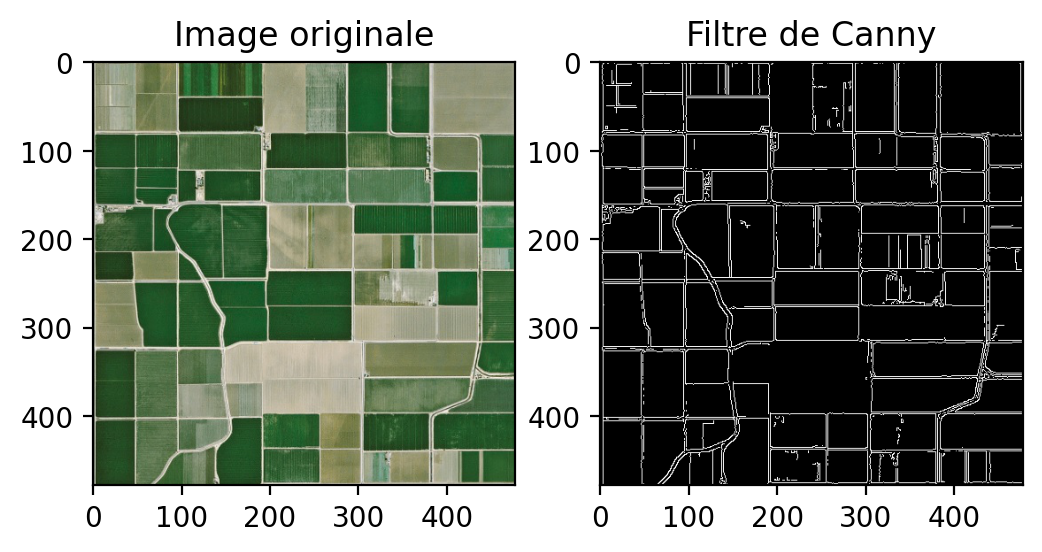
\includegraphics[scale=1.2]{canny_filter.png}
\caption{Résultat du filtre de canny}
\end{figure}



\subsubsection{Filtre de Gabor}

Le filtre de Gabor, est un filtre linéaire utilisé dans une myriade d'applications de traitement d'image pour la détection des bords, l'analyse de texture, l'extraction de caractéristiques, etc. Les caractéristiques de certaines cellules du cortex visuel de certains mammifères peuvent être approximées par ces filtres. Il a été démontré que ces filtres possèdent des propriétés de localisation optimales dans le domaine spatial et fréquentiel et sont donc bien adaptés aux problèmes de segmentation de texture. Les filtres de Gabor sont des classes spéciales de filtres passe-bande, c'est-à-dire qu'ils autorisent une certaine «bande» de fréquences et rejettent les autres. Un filtre de Gabor peut être considéré comme un signal sinusoïdal de fréquence et d'orientation particulières, modulé par une onde gaussienne.

Gabor Filter travaille sur une banque de 16 filtres à une orientation de 11.250 (c'est-à-dire si le premier filtre est à 00, alors le second sera à 11.250, le troisième sera à 22.50, et ainsi de suite.). La figure suivante montre tous les filtres de 16 filtres :


\begin{figure}[H]
\centering
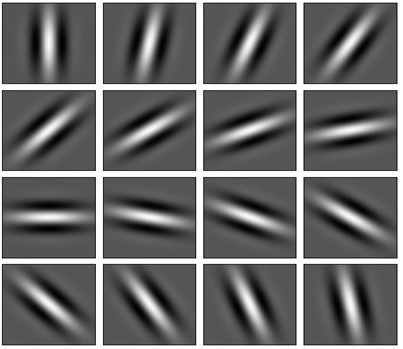
\includegraphics[scale=0.9]{gabor_16_filtres.jpg}
\caption{Banque de 16 filtres de Gabor}
\end{figure}

Pour mieux comprendre ce que chaque filtre détecte dans l'image d'entrée, considérons un simple cercle blanc sur fond noir. Lorsque cette image passe à travers chaque filtre de la banque de filtres, le bord du cercle qui est détecté est le bord orienté selon un angle auquel le filtre de Gabor est orienté. La figure suivante le montre clairement :

\begin{figure}[H]
\centering
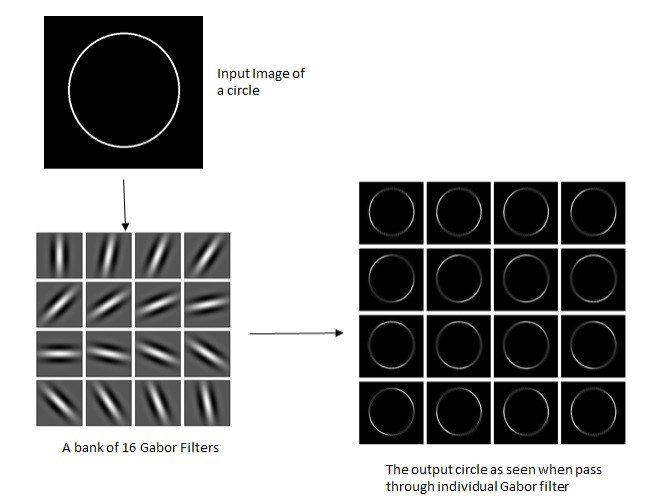
\includegraphics[scale=0.9]{gabor_method.jpg}
\caption{Exemples de détéction de contours pour le filtre Gabor}
\end{figure}

Voici la structure de la fonction qu’on a utilisée pour créer un noyau Gabor: 


\makebox[\textwidth]{
    \textbf{cv2.getGaborKernel(ksize, $\sigma$, $\theta$, $\lambda$, $\gamma$, $\psi$, ktype)}
    }
Avec :
\begin{mylist}
\item ksize : la taille du noyau Gabor. 
\item $\sigma$ : l'écart type de la fonction gaussienne utilisée dans le filtre de Gabor.
\item $\theta$ : l'orientation de la normale aux bandes parallèles de la fonction de Gabor.
\item $\lambda$ : la longueur d'onde du facteur sinusoïdal dans l'équation ci-dessus.
\item $\gamma$ : le rapport d'aspect spatial.
\item $\psi$ : le décalage de phase.
\item ktype : le type et la plage de valeurs que chaque pixel du noyau Gabor peut contenir.
\end{mylist}

Voici notre résultat en appliquant le filtre de Gabor : 


\begin{figure}[H]
\centering
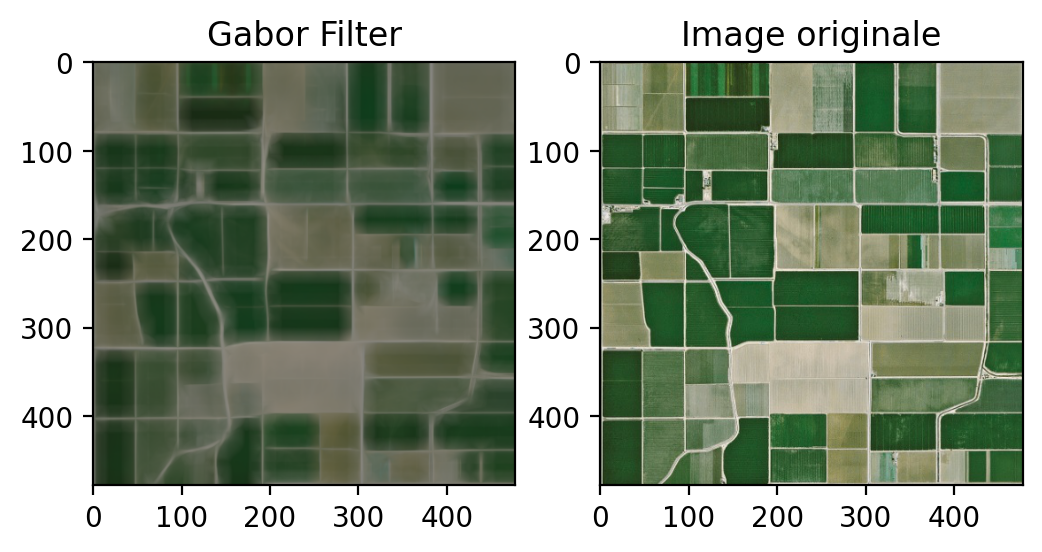
\includegraphics[scale=1.2]{gabor_result.png}
\caption{Filtre de Gabor}
\end{figure}

\section{Résultat final}

On a utilisé une image satellite de taille 478*478, on a commencé par appliquer un simple filtre gaussien pour diminuer le bruit afin d'appliquer une ségmentation bien précise on a donc choisi SVM afin de définir nos propres classes et obtenir un résultat plus clair, par la suite on a essayé d'appliquer un filtre de Canny à l'image originale pour détécter les contours des parcelles, ensuite on a fait une dilatation à ces contours pour qu'ils soit fermés et mieux cohérant, voici le processus pour obtenir le résultat final: 

\begin{figure}[H]
\centering
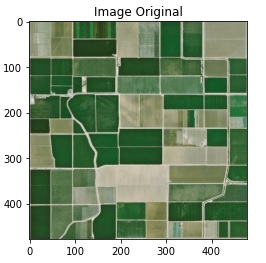
\includegraphics[scale=1]{imgor.jpg}
\caption{L'image originale}
\end{figure}

\begin{figure}[H]
\centering
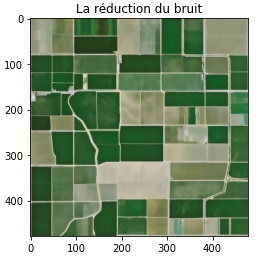
\includegraphics[scale=1]{blur.jpg}
\caption{La diminution de bruit avec un filtre de Gauss}
\end{figure}

\begin{figure}[H]
\centering
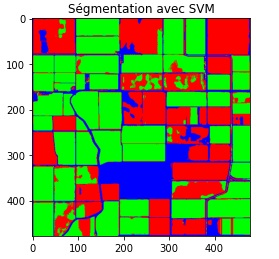
\includegraphics[scale=1]{svm.jpg}
\caption{La ségmentation avec SVM}
\end{figure}

\begin{figure}[H]
\centering
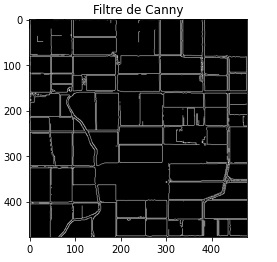
\includegraphics[scale=1]{canny.jpg}
\caption{La détéction des contours avec Canny}
\end{figure}

\begin{figure}[H]
\centering
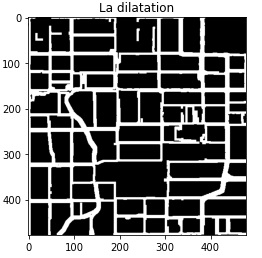
\includegraphics[scale=1]{dilation.jpg}
\caption{La fermeture des contours avec l'application de la dilatation}
\end{figure}

\begin{figure}[H]
\centering
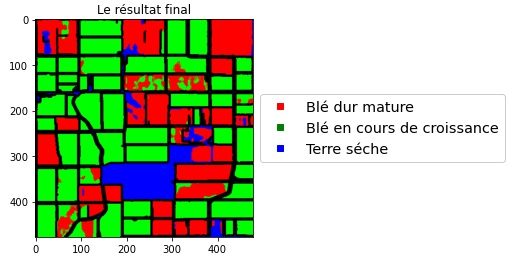
\includegraphics[scale=1]{final.jpg}
\caption{Le résultat final}
\end{figure}



\chapter*{Conclusion}
Dans un environnement qui avance et se modernise au rythme de la technique et des innovations digitales, il ne fait aucun doute que le big data et l'Internet des objets, entre autres, changeront progressivement le visage de l'agriculture. C’est déjà le cas aujourd’hui. La poursuite de la digitalisation de l'agriculture sera un pas en avant indispensable dans le monde de l'agriculture moderne.
\par
Ainsi le crop Mapping peut assurer la sécurité alimentaire et éviter les pénuries potentielles dans la chaîne d'approvisionnement alimentaire en identification des cultures en temps quasi réel avec la précision exceptionnelle obtenue grâce à l'utilisation des données satellitaires.
\par
Bref, ce projet nous a permis d’appliquer les connaissances qui nous ont été inculquées au cours de cette année et de découvrir de nouveaux concepts et domaines traitement des images mais aussi du deep learning à travers les algorithmes utilisés pour la segmentation.
Il nous a permis aussi de développer nos aptitudes de travail en équipe, de communication et de résolution des problèmes qui ont surgi lors du déroulement du projet.



%Bibliographie_______________________________________________________

\begin{thebibliography}{9}


\bibitem{frag}
Agriculture et Biodiversité en Bretagne\\
\textit{Freagmentation du parcellaire}. \\
\url{http://www.agriculturebiodiversite.fr/ameliorer-la-biodiversite/amenager-son-exploitation/fragmentation-du-parcellaire.html}

\bibitem{imagesatt}
Les images et les statistiques concernat le Maroc\\
\textit{Centre Royal de Télédétection Spatiale}.\\
\url{https://www.crts.gov.ma/thematiques/agriculture/suivi-d-etat-des-cultures}

\bibitem{agr}
Agriculture en chiffres 2018 (édition 2019)\\
\textit{Ministère de l'Agriculture, de la Pêche Maritime, du Développement Rural et des Eaux et Forêts}\\
\url{http://www.agriculture.gov.ma/pages/publications/agriculture-en-chiffres-2018-edition-2019}

\bibitem{orbite}
Combien de satellite tournent autour de la Terre ?\\
\textit{Céline Deluzarche, Publié le 12/04/2020, FUTURA SCIENCES}\\
\url{https://www.futura-sciences.com/sciences/questions-reponses/satellite-satellites-tournent-autour-terre-7065/}

\bibitem{sentinel}
Sentinel missions\\
\textit{The European Space Agency, Observing the Earth}\\
\url{http://www.esa.int/Applications/Observing_the_Earth/Copernicus/Overview4}

\bibitem{ref3}
Les informations contenues dans une image, analogique ou digital ?\\
textit{ESA (European Space Agency) eduspace, 2015}\\
\url{https://www.esa.int/SPECIALS/Eduspace_FR/SEM11YR7NWF_0.html?fbclid=IwAR1DA8wJKDujA2pHMdAoyIz54p5T6kFdVWR6EkySLQCe5O98j66p2ob9LSQ}

\bibitem{ref4}
Comprendre une image satellitaire\\
\textit{GéoBretagne Publication de 2016}\\
\url{https://cms.geobretagne.fr/content/comprendre-une-image-satellitaire?fbclid=IwAR1kR644UcZJa0bt_ZamhZt5UldAfCv-Na9Cto6f2yS-5eiIkAgjWaclgc0}

\bibitem{satt} 
Les satellites au service de l'agriculture\\
\textit{Article de Rémy Decourt publié le 4 avril 2011}.\\
\url{https://www.futura-sciences.com/sciences/actualites/astronautique-satellites-service-agriculture-29034/}

\bibitem{cropmapp}
Generating Crop Classification Maps Using AI\\
\textit{David Markowitz, 6 May 2019, Planet Watchers}\\
\url{https://www.planetwatchers.com/generating-crop-classification-maps-using-ai}

\bibitem{modis}
MODIS Vegetation Index Products\\
\textit{Kamel Didan, Moderate Resolution Imaging Spectroradiometer, NASA}\\
\url{https://modis.gsfc.nasa.gov/data/dataprod/mod13.php}

\bibitem{deeplearning}
Deep Learning Classification\\
\textit{ IEEE Geoscience and Remote Sensing Letters ( Volume: 14 , Issue: 5 , May 2017 }\\
\url{https://ieeexplore.ieee.org/abstract/document/7891032?fbclid=IwAR3TiBL273ykf0RpPCORrCK0hayB4ePCgp21eh76O0cBOBMBszCdKtk2E1g}

\bibitem{k-means definition}
Tout ce que vous voulez savoir sur l’algorithme K-Means\\
\textit{Younes Benzaki, blog Mr. Mint,  10 avril 2018}\\
\url{https://mrmint.fr/algorithme-k-means}


\bibitem{k-means}
K-means Clustering Python Example\\
\textit{Cory Maklin, Medium, Dec 28/2018}\\
\url{https://towardsdatascience.com/machine-learning-algorithms-part-9-k-means-example-in-python-f2ad05ed5203}

\bibitem{otsu}
Méthode d'Otsu\\
\textit{{W}ikipedia{,} The Free Encyclopedia}\\
\url{https://fr.wikipedia.org/wiki/M\%C3\%A9thode_d\%27Otsu}

\bibitem{comparaison}
Comparing Edge Detection Methods\\
\textit{Nike Tsankashvili, 20 Jan 2018, Medium}\\
\url{https://medium.com/@nikatsanka/comparing-edge-detection-methods-638a2919476e}




\end{thebibliography}

\end{document}








